\documentclass{article}
\usepackage{graphicx} % Required for inserting images
\graphicspath{ {./images/} }

\title{MS-CS Master Course Note (Non-Credit)}
\author{Mark Zhou}
\date{March 2024}

\usepackage{setspace}
\usepackage{listings}
\usepackage{amssymb}
\usepackage{xcolor}
\usepackage{float}

\setlength{\intextsep}{1cm}

\begin{document}
\maketitle
\doublespacing

\paragraph{This is my course note on “Algorithms for Sorting, Searching and Indexing” provided by Colorado University of Boulder. 
This is a non-credit prep course for an MS-CS degree.}

\newpage
\tableofcontents
\newpage

\section{Asymptotic Notation: Big O}

\subsection{Time and Space Complexity}

\paragraph{We have some questions regarding how to figure out which algo is faster.\\
Q1: what input should we choose.\\
Q2: how to evaluate time.\\
When considering implementation details, that is under the realm of performance analysis. We don't want to be bogged down to this level and only wish to focus on the algorithm.\\
The runtime is the number of basic operations. For each sorting algorithm, there will be a range of possible runtime, due to the differences between inputs, the best case, average case, and worst case respectfully.\\
The average time cost is hard to analyze while may be more desirable than the worst case cost, which is too pessimistic in some cases. Never use best case cost.\\
In most of cases we will use worst case cost to evaluate.\\
Let's assume the cost of Insertion Sort is $f(n)$.\\
Hypothetically (just for examples) speaking:\\
$ f(n) = 0.05n^2 + 1.5n +70 $\\
We assume that the different algorithms such as addition or multiplication have the same unit cost, that is to say, they cost the same under one unit run. But is that the real case?\\
Of course not. Different operations have different costs for a unit run. To change that, we can change the coefficient of the original equations.\\
We care about which algorithm is faster asymptotically. This is why this kind of analysis is called asymptotic analysis.\\
The naming is inspired by one idea, that is the comparison should be within the realm of actual usage, for instance, when sorting 10 numbers, algo1 may be slower than algo2, but while sorting 10000 numbers, algo1 may outfast the opposite, that's why we compare them asymptotically.\\
And to be aware, we focus more on cases with large numbers or unit cases than small samples.}

\subsection{Big O}

\paragraph{$ f = O(g(n)) $\\
Meaning: $f()$ is ASUMPTOTICALLY upper bounded by $g(n)$\\
Here are some properties:\\
When $g()$ overtakes $f()$, meaning in the chart, g is above f after some time, and then f will remain overtaken forever.\\
The constant factor must be disregarded.\\}

\begin{quote}
    Note: In mathematics (logic), the symbol $\exists$ is read as “there exists” and the symbol $\forall$ is read as for all.\\
\end{quote}

\paragraph{$ \exists k>0,N_0, \forall n \geq N_0, f(n) \leq k*g(n) $\\
$f(n) \leq k*g(n)$ only happens beyond some point in time. When the above condition happens, we say:\\
$ f(n) = O(g) $\\
Let's take some examples:\\
$ f=(1/2)n^2 $\\
$ g=0.1n^3 $\\
Assuming k=10, and $N_0$=1\\
Using the equation above $f(n) \leq k*g(n)$, then we will have $f(n) \leq g(n)$, which has got rid of the constant k;\\
Then we can say,\\
$f(n) = O(g) $\\
a.k.a. \\
$0.5n^2=O(0.1n^3) $\\
As long as $g(n)$ will overtake $f(n)$ after K, $g(n)$ will be the cost of $f(n)$, aka $f(n)=O(g)$.\\
Under such circumstances, adding some constants to the equation of f and g, won't change the fact that $f(n)=O(g)$.\\
The $g(n)$ must always be less than or equal to $f(n)$ to make $f(n) = O(g)$ valid: 
that is to say, after a certain point $N_0$, the output of the function $f(n)$ is less than or equal to the output of the function $g(n)$.}



\section{Big Omega, Big Theta, and Examples}

\subsection{$f(n)=\Omega(g)$}

\paragraph{f is asymptotically lower bounded by g (n): that is to say, after a certain point $N_0$, 
the output of the function f (n) is bigger or equal to the output of the function g (n).Since O () and $\Omega()$ are the opposite, if f (n) = O (g), then $g(n)=\Omega(f)$.}

\subsection{$f(n)=\Theta(g)$}

\paragraph{f is asymptotically equal to g (n). This looks like a Bollinger band in technical analysis in some ways.\\
$\exists k_1,k_2, \forall n \geq N_0,k_1(g) \geq g \geq k_2(g)$\\
If $f = \Theta(g)$, it means f is asymptotically equal to $\Theta(g)$, which we can say,\\
$f = O(g),  f = \Omega(g)$\\
When dealing with functions, we will typically get rid of constant figures in the function, however,\\
we cannot ignore the exponent constant such as the 2 and 4 in 2 to the power of 4x. \\
$2^{4x}$\\
Here is an example of big theta.\\
$f(n)=2n+3\log_2^n+5$\\
$g(n)=15n+35\log_2^n+\sqrt{n}+17$\\
In the above equations, n is the only thing that matters. Therefore we can ignore the log and square root elements by considering them as constants.}

\subsection{Examples of Asymptotic Notations}

\paragraph{Here are five functions;\\
$f(n)=2n^2 + 3\log_2^n + 4\sqrt{n} + 15$\\
$g(n)=200\sqrt{n} + 15\log_2^n + 14n\sqrt{n}$\\
$h(n)=n^2 + 2n + 3\log^{logn}$\\
$l(n)=n^3 + 15n^2 + 2.5n$\\
$m(n)=4n^2 + 13n^2\log_2^n$\\
Let's find out which element with n is the BIGGER one.\\
$n^2=n*n > nlogn > \sqrt{n}$\\
Before we can compare these functions, we should determine the dominating term of each one:\\
$f: n^2$\\
$g: n^{1.5}$\\
$h: n^2$\\
$l: n^3$\\
$m: n^2logn$\\
In this case, we can place these functions in such order,
$l > m > f > h > g$\\
The smaller one is the Omega of the bigger one, and vice versa.
For example, $l(n)=\Omega(m)$, $m=O(l)$, and so on.}


\newpage

\section{Binary Search}

\subsection{what do we need to do in a binary search?}

\paragraph{We need to check if a given element, say 6, is located in the given list. The prerequisite is that the list must be sorted to do a binary search.\\
Let's assume the list is sorted in ascending order. First, we need to find the middle element of the list by calculating the index number of left and right border elements, a.k.a. the first and last one in the list.\\
Here is how we do it:\\
$mid=(left + right) // 2$\\
In the equation, // means floor divided, which will return exact the middle element with odd number list and the smaller one of the middle two elements in even number list.\\
Now we will check if the middle one equals to the given element. If so, problem solved! If not, and the given one is smaller than the middle, we will focus on the left side of the list, a.k.a. the elements located on the left of the middle one. 
In this case, if the first middle has index n, then the new “right” border element will have the index n-1.\\
If the middle element is smaller, of course we will focus on the right portion of the original list since this is an ascendibg ordered list. And in this case, if the first middle element's index is n, the new “left” will have the index n+1.
Then we will conduct the calculation by finding the new middle on the left/right part of the list (a.k.a. the new range with the updated left or right border). We will compare the given value with the new middle.\\
We will repeat the process untill either find the element in the list, returning True, or not, which is a little bit complecated:\\
By the end of the process, the updated left border index will be bigger than the right border index in an ascending ordered list, which is not possible to find a valid range. This means the given element is not in the list.\\
For example, there is a list [1,4,9,15,20], and the given element is 8.\\
First we will find out the mid one by calculating the indexes:\\
$(0+4) // 2 = 2$\\
 The value of index 2 is 9, which is bigger than the given value 8. Then we will focus on the left part.\\
The updated right border will be index 1, therefore the new mid will be:\\
$(0 + 1) // 2 = 0$\\
Now the equation gives us element value 1. This is smaller than 8. The current right border index is 1, and the updated left border is 1 as well. So the new range will gives us;\\
$(1 + 1) // 2 = 1$\\
a.k.a. the value of index 1 is 4 which is smaller than 8.\\
And now we enter a crucial moment. The current right border index is 1, but since $4 > 8$, the updated left border index will be changed from 1 to 2.\\
Left index=2, right index =1, which is not valid.\\
Therefore, the given element 8 is not located in the given list. Problem solved.}

\subsection{Define a Func binarySearchHelper()}

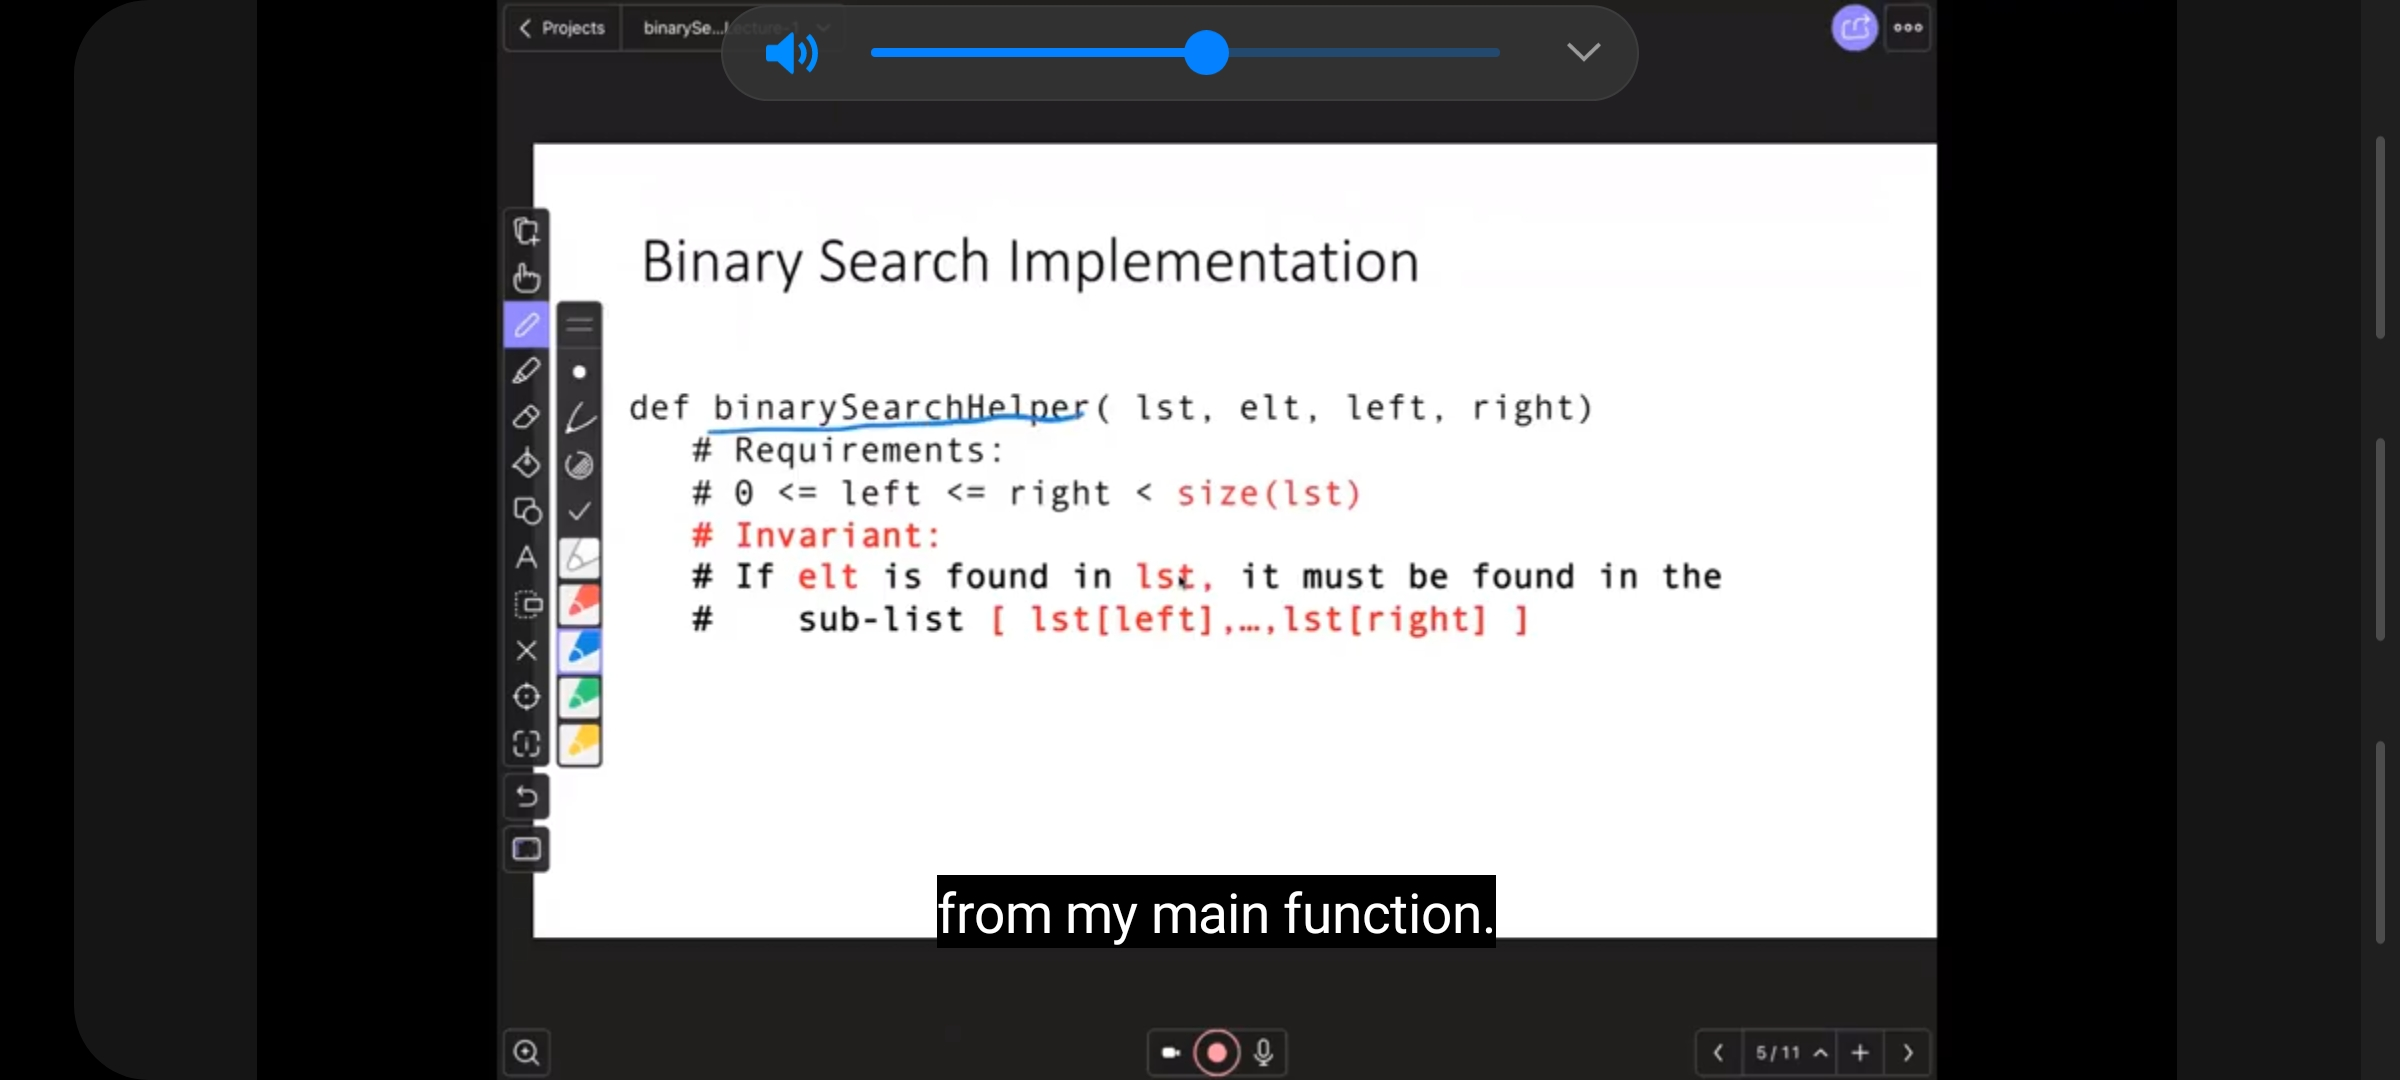
\includegraphics[width=\textwidth]{binarysearchhelper}



\paragraph{Here is the code implemented of the fuc binarySearchHelper().\\
This function will work as a recursion since it will continuously call a new binarySearchHelper() inside the current one until finished.\\
How to prove correctness?\\
The main property of binary search: if we can find the element in the list, it must be in the searching range.}

\subsection{Running Time Analysis of Binary Search Algo}

\paragraph{For the running time analysis, we first assume this list has the length of:\\
$n = 2^k$\\
Each time when we check the middle element, we halve the list in half, then the updated list will have a new lengh of\\
$n/2 = 2^{k-1}$\\
By the end, the list will have a length of\\
$2^{k-k} = 1$\\
Now we narrow down the checking range to only one element and check it with the given value. If they are not the same, we will try to find a new middle for more time, which will produce an invalid range as we mentioned before.\\
That is to say, we will at most run the program k+1 times until finished. So by the end, the largest running time will be: \\
$\log_2^n + 1$\\
Binary search is very efficient. If we have a list of 1 million values, we may only need to search for approximately 21 times.}


\newpage

\section{Merge Sort}

\subsection{Mergesort: Correctness and Running Time}

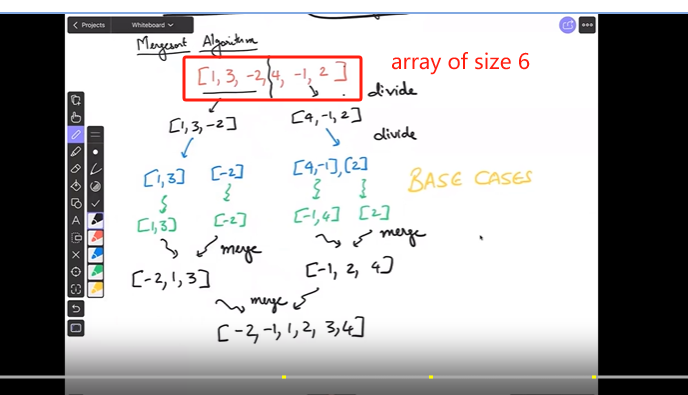
\includegraphics[width=\textwidth]{mergesort}



\paragraph{In order to do a mergesort, firstly we will divide the given array into two parts with the middle element as a separator.\\
For example, we have an array \[1,3,-3,4,-1,2\]\\ We will divide it into \[1,3,-2\] and \[4,-1,2\]\\
Then we will further divide these two into four parts. By now, we have some array contain one one item while others contain two. For those with two items, we will do a swap if they are in the wrong order.\\
These kinds of very small divided array are called base cases, since they are somehow the base unit of this division process.\\
Then we will merge back all those sorted base case arrays, all the way to the top, aka one merged array.\\}


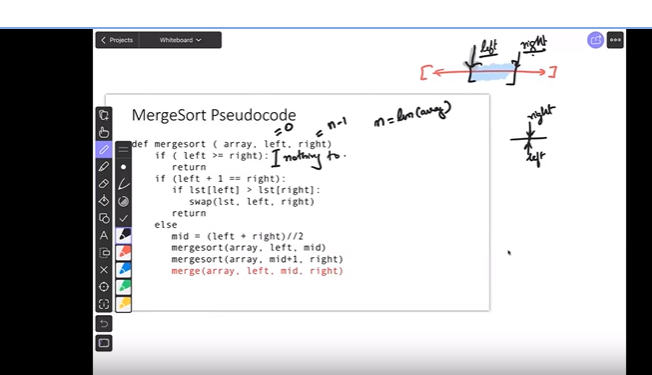
\includegraphics[width=\textwidth]{mergesortpseudocode}


\paragraph{Here is a pseudocode of mergesort. Let's get a closer look at how does it work.\\
At the very beginning, the algo will compare left and right element and check if they are in a valid form, that is to say, whether left (index of the value) is smaller than right (index of the value). If not, the range formed by the left and right index is invalid hence algo ended.\\
Second, we will determine whether the array formed by left and right contains only two elements. If $left + 1 = right$, that means these are adjacent indices. If this is the case, we will swap the elements if they have the wrong order.\\
At last, we enter a position in which the range is larger than two elements array. Now we will simply find the mid element by performing a floor division and do merge sort on left side of the array which is ended by mid and right side which begins with mid+1. 
This procedure will sort this two subarrays. After that, we will MERGE all the subarray in the order of left, mid and right.\\}

\paragraph{The merge procedure is the next big thing. After this step, all the elements of the array will be sorted. \\
First thing in Merge function, we will assign an initial value to two looping variables, i and j, which are the index of each subarray, by assigning left to i and mid+1 to j. This is to make sure the two loops will begin from the first item of each sub array, aka the left array and right array.\\
We will introduce a temp storage variable \texttt{tem\_store} to maintain the sorted result and then write back to the original array. Although there are in-place algos that will do the work, it is much easier to just include a third array for storage.\\
The following is straight forward. While i and j are still within the range of each subarray, aka $i \leq mid$ and $j \leq right$, we will compare each i and j pair and store the smaller one to the \texttt{tem\_store}. 
Then we add one to the index of the subarray in which the value just compared is smaller, that is to say, move on to the next item. In the meantime, the other array remain the same index, waiting to compare in the next round.\\
After all these steps and iterations, we will find a well sorted \texttt{tem\_store} array. Then we simply write it back to the orginal array and problem solved.}

\subsection{Running Time of Merge Procedure}

\paragraph{The running time of merge procedure is precisely the length of the two arrays since each element will be added to the temp store once. We assume each step cost 1, then the total time cost will be len(array A+array B).\\
It can be written as $right - left + 1$.\\
Now let's look at it at higher level.\\
Suppose the original array has lenth of n.\\
The first split will be two n/2 arrays, then the split goes on until it reaches the base unit.\\
For each step, the cost will be the array's count mutiply by the base unit, for example, for the 1st level, the cost will be $2*(n/2)$, for the 2nd, it will be $4*(n/4)$ and so on.\\
Now we can try to conclude a general equation for the time cost of merge sort.\\
Let us assume that $n = 2^k$;\\
Since for each level, the number of level is $n, n/2, n/4, \ldots ,1$;\\
We can write it as $2^{k-1},2^{k-2}, \ldots ,2^{k-k}$.\\
For each level, the time cost is the base unit of that level mutiply by that level's amount of subarrays in that level. For example, the base unit of the 1st level after n is n/2. Then the time cost will be $2 * (n/2)$.\\
Therefore, the generalized time cost will be $n * No.(level)$. Now let's find out what's the number of level. \\
We have already seen this above: $2^{k-1},2^{k-2}, \ldots ,2^{k-k}$, corresponding to level 1, level 2, \textellipsis, last level. We can derive the number of level from this array, $1,2, \ldots ,k$.\\
That is to say, the number of level is k. Ergo $n * No.(level) = n * k$.\\
Since $n = 2^k, k = \log_2^n$.\\
The final equation will be:\\
$Cost = n * \log_2^n$\\
If we using the Big O quatation to address to this problem, we get\\
$Mergesort = \Theta(n * \log_2^n)$\\
And we can get rid of the constant 2 and get\\
$Mergesort = O(n * \log^n)$.}


\newpage

\section{Heap, Min Heap and Max Heap}

\subsection{Basic Understanding of Heap}

\paragraph{Heap is a type of array that has certain properties. There are the concepts of min heap and max heap and we will go through these soon.\\
First here's a concept called left/right child. Let's say we have a heap of 9 elements. For element number 1, the element number 2 will be called the left child of element 1, and element 3 will be called the right child.\\
While for element 2, actually element 4 will be the left child and 5 the right child.\\
Therefore we have the equation of it:\\
$\forall i,leftchild = 2i,rightchild = 2i + 1$\\
For certain element in the array, If the left/right child element is not inside the current array, then the original one doesn't have left/right child.\\
For example, element 6 has not such child since element 12 and 13 are not in the array of size 9.\\}


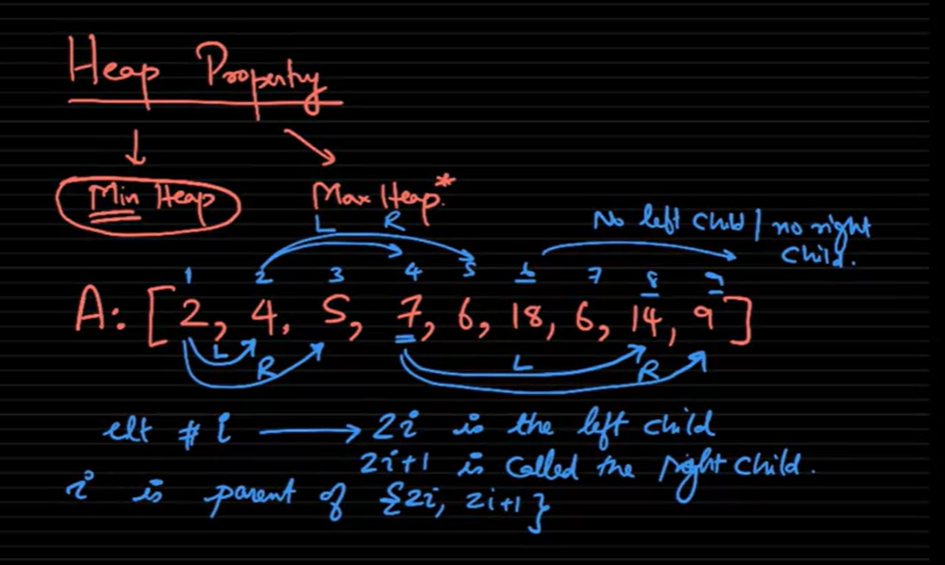
\includegraphics[width=\textwidth]{heapproperty}



\paragraph{We can say i element is the parent of 2i and 2i + 1.\\
for element j, j/2 is the parent. If the division gives a fraction of number then we just round it down (floor division).\\
Element 1 has not parent, and we call it the root.\\}

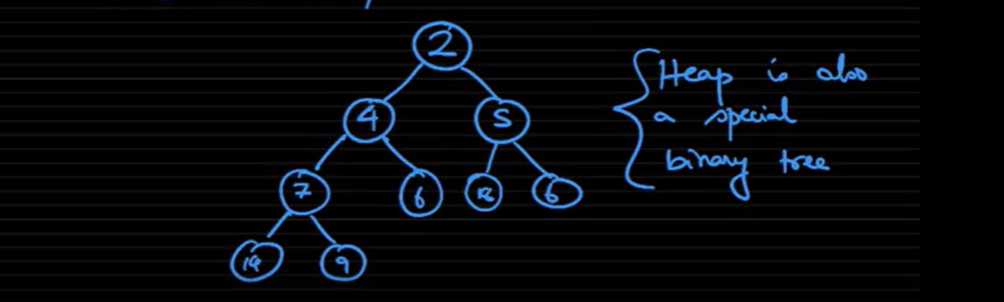
\includegraphics[width=\textwidth]{heapbinarytree}



\paragraph{If we write the heap array in a parent-child structure, it actually looks like a tree. Yes, heap is also a special binary tree (laid out as an array).\\
Here are some properties:\\
1. If a node in a heap has a right child, it must have a left child.\\
2. Heap is an array of size n. $\forall A[i],2i \leq n,A[2i] = leftchild$\\
3. $\forall A[i],2i+1 \leq n,A[2i+1] = rightchild$\\
And here is the Min Heap Property:\\
The value of the parent node must be less than or equal to the value of children nodes.\\
Min Heap → $ParrentValue \leq ChildrenValues$\\}


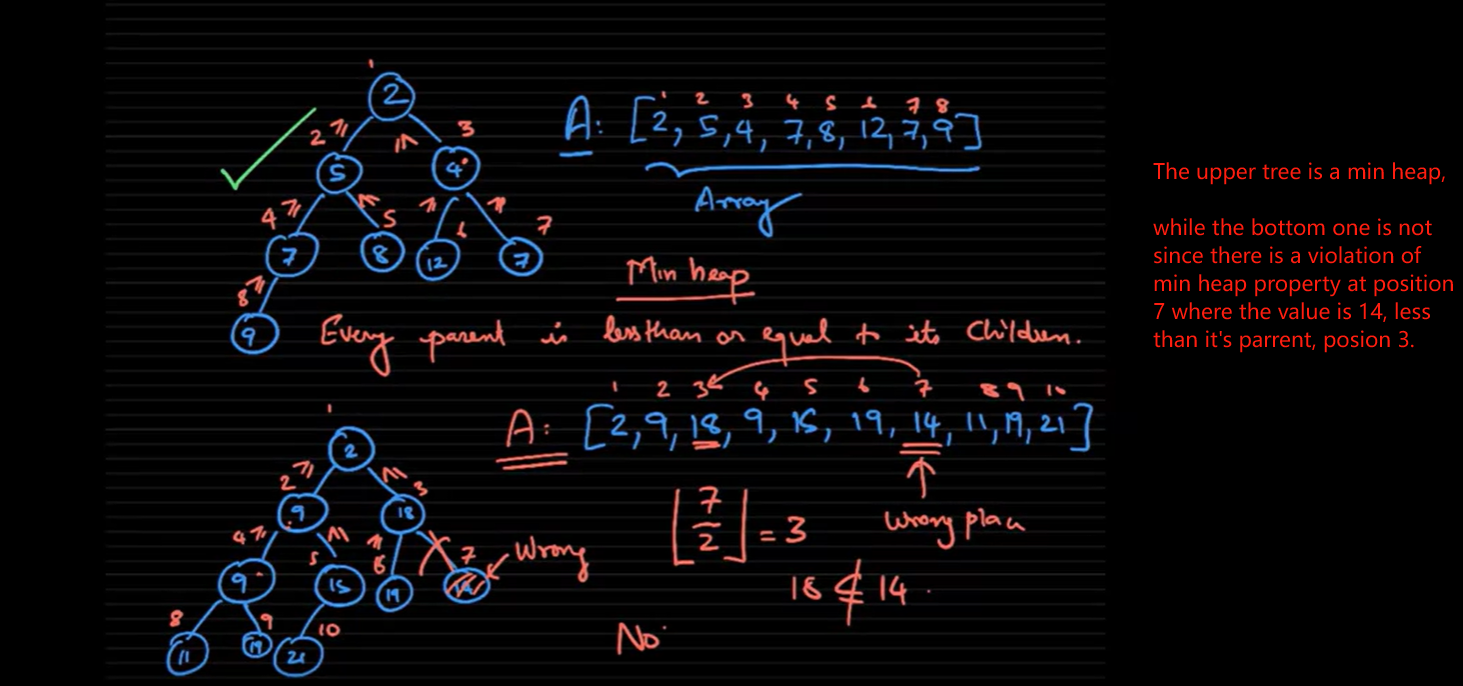
\includegraphics[width=\textwidth]{minheap}



\paragraph{If we turn to the opposite side, we get the Max Heap Property: The value of the parent node must be larger than or equal to the value of children nodes.\\
Max Heap → $ParentValue \geq ChildrenValues$\\
So for any array, we can simply check whether they meet min heap property or max heap property or not in order to determine their identity.\\
Why do we care about min heap or max heap? Here is a basic idea;\\
For any min heap A, we can say A[1], which is the root, is the smallest element of the entire array.\\
We can solve this problem with induction.\\
The Base Case: The root element is the smallest one for Heap depth = 1.\\
And we have the induction hypothesis: Let the result from base case hold for all $depth \leq d$, and then prove it for depth of d + 1.\\
Illustrated as a binary tree, we can see each triangle (consisting of three nodes) as a “sub-heap”. The node in the upper level of the sub-heap is the root of it. 
For every level from 1 to d, the upper node is always the root of each sub-heap. Therefore the root of level 1 is the smallest in all level from 1 to d.\\
Then we can say that's the same case for level d+1.\\
That is to say, for any min heap A, we can say A[1], the root of it is the smallest element of the entire heap.}

\subsection{Heap Primatives: Bubble up}

\paragraph{We are interested in the following operations on a heap:\\
1. Inserting elements into a heap\\
2. Deleting one from a heap\\
The main primitives of heap are called bubble up and bubble down. We will explain them later.\\
For now, lets assume there is a heap with only one point of failure. Here is an example of such min heap.\\
In the above array, the 6th element, which value is also 6, is smaller than its parrent element 3, with a value of 7. Besides that, the entire array fit the definition of min heap.\\
We can say in this case, the 6th element is in a wrong relation with its parent. It should be moved up in order to make this array a valid min heap.\\
The operation that will acheive this is called bubble up.\\
Bubble Up: the swap of a value with its parrent value if they are in the wrong relation.\\
After we sway the misplaced value with its parent, now we have a new parrent of value 6 and its left child 7. Since the parrent is also less than or equal to its right child. The array is now a valid min heap.\\
Here is another example. We need to bubble up 3 times in order to make it a min heap.\\
\[2,3,7,4,5,9,11,1,8\]\\}


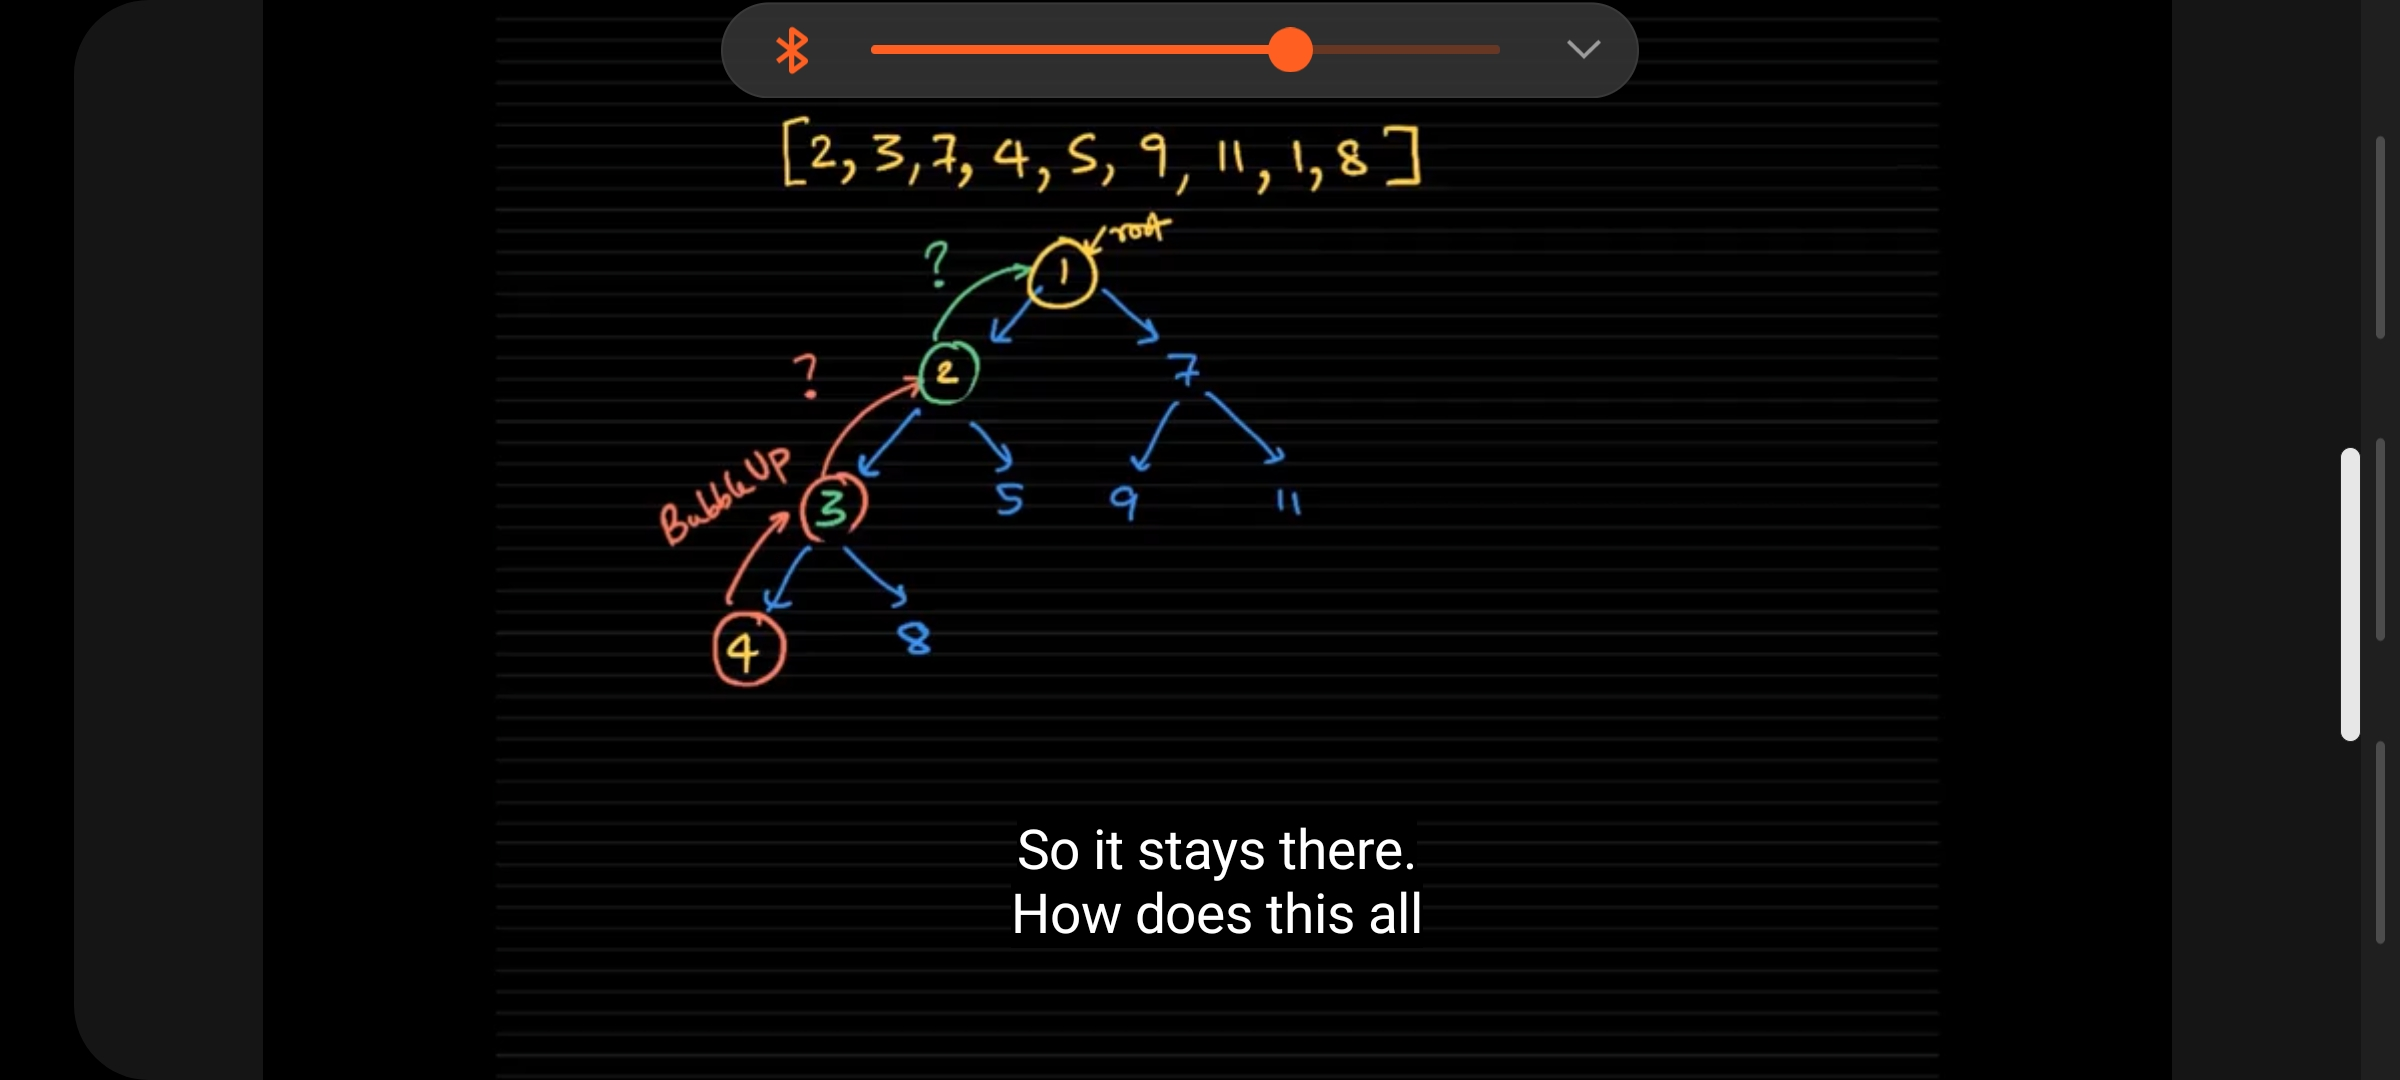
\includegraphics[width=\textwidth]{bubbleup}



\paragraph{In the above array, every elements except the last but one are in the right position. Element 8 with value of 1, is smaller than its parrent.\\
Then we need to bubble up value 1 three times into position 4, 2, and 1 to make it work. Now value 1 become the root.\\
We can write a pseudocode for bubble up:\\}

\begin{verbatim}
    bubble up (A,j):
        if $j \leq 1$:
            return (Do nothing)
        else if:
            $A[j] < A[j//2]$: (// means floor divided)
            swap (A[j], A[j//2])
            bubble up (A,j//2) 
            #Yes, this line makes this function recursive.
        return
    \end{verbatim}

\paragraph{This is a recursive program that will bubble up the misplaced element until it is in the right place.If we try to estimate the running time of bubble up, the worse case would be O (depth of heap), since the element will be a leaf (the one without child) and it lays on the bottom level of the heap.\\
Then how about $\theta$? Let's assume a heap has n element. If the leaf needed to be bubble up all the way to root position, the steps will be:\\
$n,n/2,n/4, \ldots ,1$\\
Then the steps will be $\log_2^n$, a.k.a. $\theta(\log_2^n)$.\\
If we have a heap of $n = 10^6$, which is $2^{19}$, then the total operation required for bubble up is 19.}

\subsection{Bubble Down}


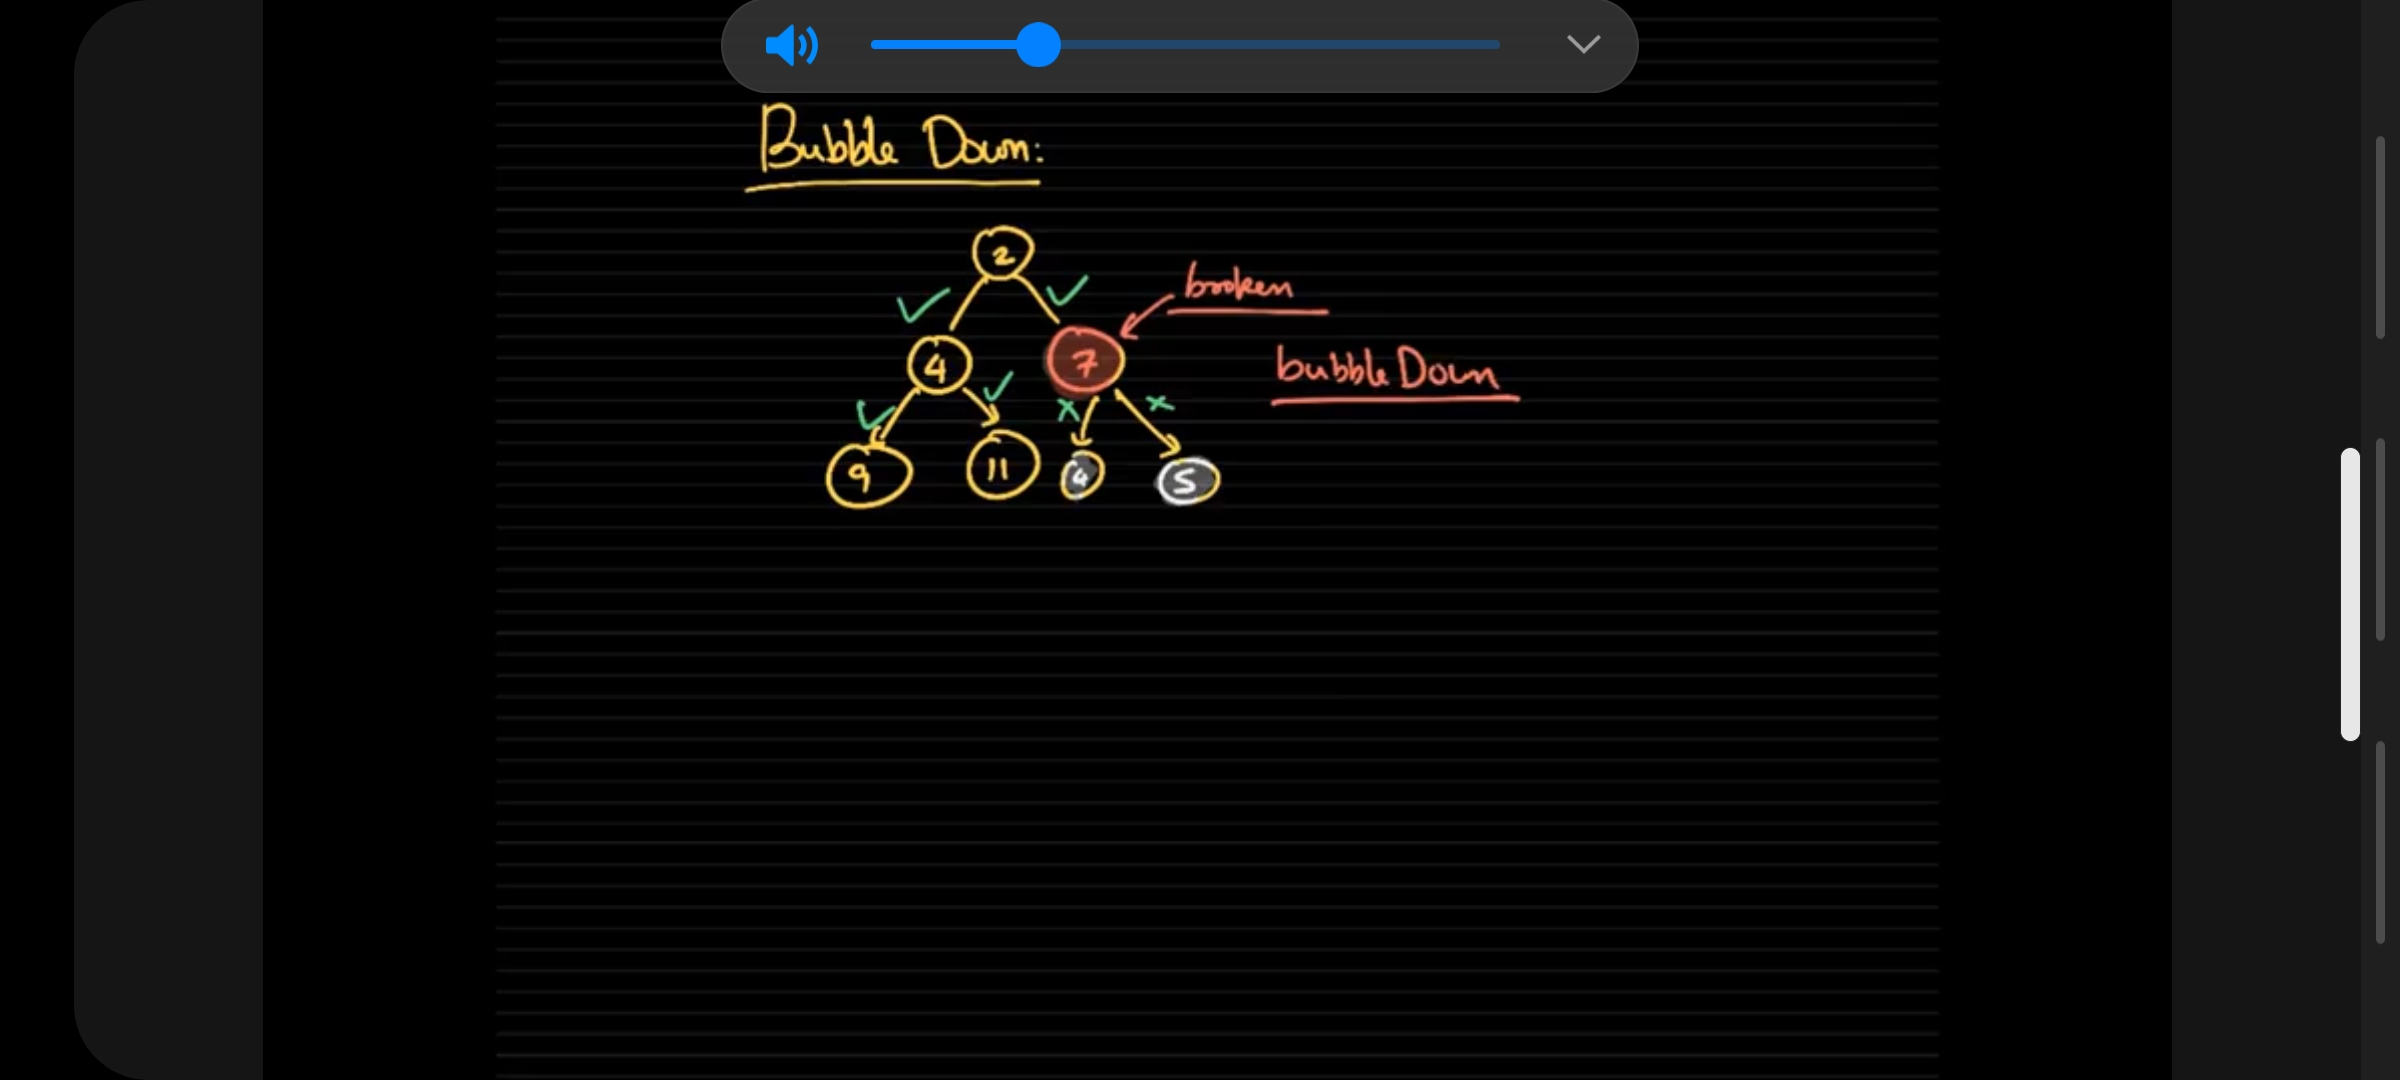
\includegraphics[width=\textwidth]{bubbledown}



\paragraph{In opposite to bubble up, bubble down is the operation that will move the root element to the right position.
That is to say, if the root element is not the smallest one, we will swap it with the smallest child.
So in the example above, the element 7, which is the parrent of 4 and 3, will be swapped with 3.\\
What if we cannot bubble down once and place the root element in the right position? Sometimes we need to do it multiple times.\\
Here is a min heap that needs to be bubbled down twice.\\}


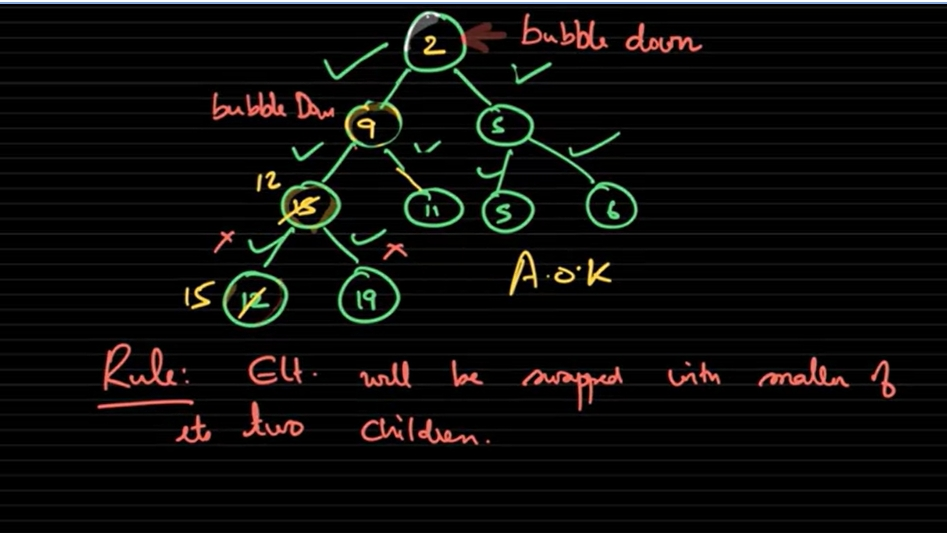
\includegraphics[width=\textwidth]{bubbledownmultipletimes}



\paragraph{Now let's take a look at the pseudocode of bubble down.\\}

\begin{verbatim}
    bubble down (A,j):
        if $2j > n$: (2j is actually the left child, n is the length of A.)
            return (Do nothing since A has no children.)
        else if: $2j \leq n$ and $2j+1 \geq n$: (no right child)
            if $A[j] > A[2j]$:
                swap (A[j],A[2j])
                bubble down (A,2j) (recusive)
        else if: $2j \leq n$ and $2j+1 \leq n$: (has both children)
            if $A[2j] \leq A[2j+1]$ and $A[j] > A[2j]$: 
            #Left child is smaller, which will be swapped with the current parrent.
                swap (A[j],A[2j])
                bubble down (A,2j) (recusive)
            else if $A[2j] > A[2j+1]$ and $A[j] > A[2j+1]$: 
            #right child is smaller and will be swapped.
                swap (A[j],A[2j+1])
                bubble down (A,2j+1) (recusive)
        return
\end{verbatim}

\paragraph{We will first compare 2j, which is the left child of j, with n, the length of A.
If $2j > n $, j has no children whatsoever. \\
Then we go into the second condition, parrent j has only one child, the left one of course.
If the parrent is bigger than its child, in this case $A[j] > A[2j]$, we need to swap them.\\
At this moment, we will need to run the recursive procedure, that is to call bubble down again.\\
The third condition is that the parrent has both children. We will compare the left child with the right child. 
If the left child is smaller, we will compare it with the parrent. If the parrent is bigger, we will swap them. 
Of course, we will need to recursively run bubble down again.\\
By the end, if the right child is smaller, we will compare it with the parrent. 
If the parrent is bigger, we will swap them and call the main function recursively.\\
Problem solved.\\}

\paragraph{How do we estimate the running time of bubble down?\\
The worst case will be the leaf node, which is the last level of the heap. That is to say, we need to bubble down the root element all the way to the bottom of the heap.\\
The time cost will be the depth of the heap, which is $\theta(\log_2^n)$.\\
How do we get this number? Let's do the math again.\\
In order to get the depth of the heap, we need to find out how many levels the heap has.
The root element which needed to be bubbled down will move through the following steps;\\
$1,2,4,8,16, \ldots ,n$\\
Which can be rewritten as $2^0,2^1,2^2,2^3,2^4, \ldots ,2^k$\\
k is the depth of the heap, and $k = \log_2^n$.\\}

\subsection{Reading Note on CLRS Chapter 6.3}

\paragraph{Heapify is the process of reshaping a binary tree into a heap data structure.\\
The main idea of min heapify is to make sure that the root of the tree is the smallest element of the entire tree.\\
The min heapify procedure is a recursive one.\\}

\subsection{Priority Queue, Heapify and Heapsort}

\subsubsection{Inserting into a heap}

\paragraph{First we need to understand how to insert an element into a heap.\\
The main idea is to insert the element at the end of the array and then bubble up the element until it is in the right position.\\
That is to say, insertion = insert to the end + bubble up.\\
The time cost of inserting to the end of the heap is just as simple as $\theta(1)$.\\
Then we need to bubble up the element. The time cost is $\theta(\log_2^n)$.\\
So the total time cost is just $\theta(\log_2^n)$.\\}

\begin{figure}[h]
    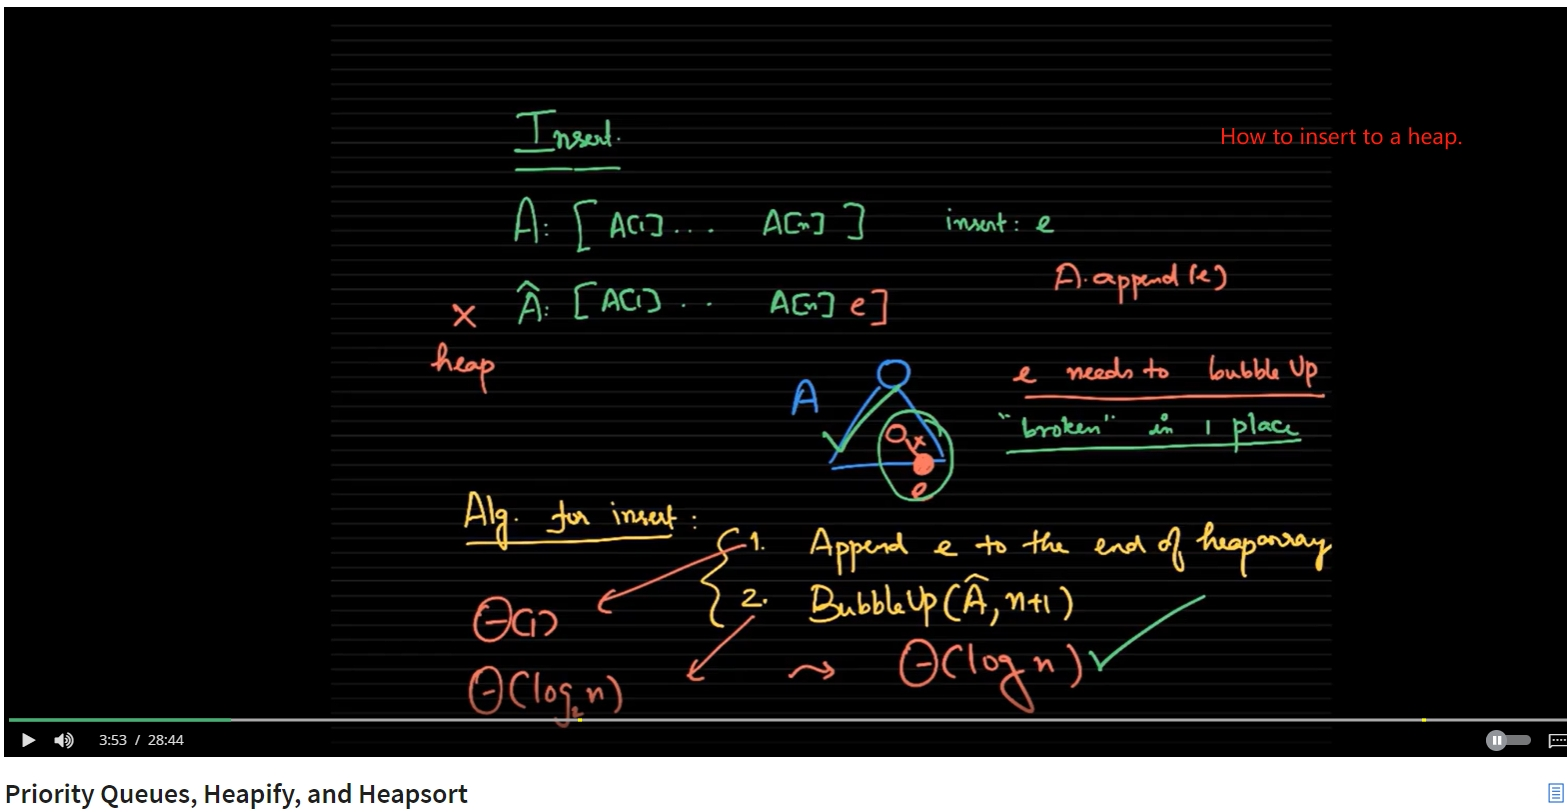
\includegraphics[width=\textwidth]{inserttoaheap}
\end{figure}


\subsubsection{Deleting from a heap}

\paragraph{Then we come to the concept of deletion of a heap element.\\
1. Replace the element that we want to delete with the last element of the heap.\\
2. Adjust the lenth of the heap to n-1, assuming the original length is n. Now we can simply delete the last element.\\
3. Bubble up or bubble down the element that we moved. The specific operation we use depends on the situation. We need only one operation for any cases.\\}

\begin{figure}[h]
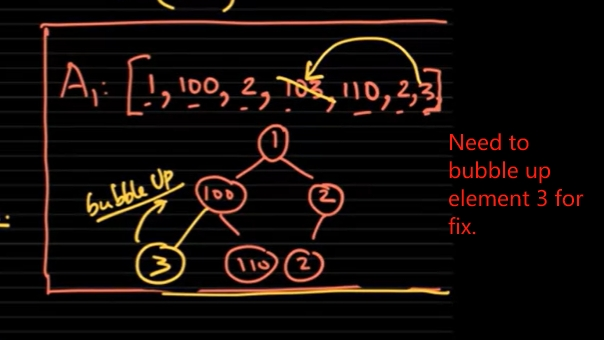
\includegraphics[width=\textwidth]{bubbleupafterdeletion.png}
\caption{Bubble up for a fix.}
\end{figure}

\begin{figure}[h]
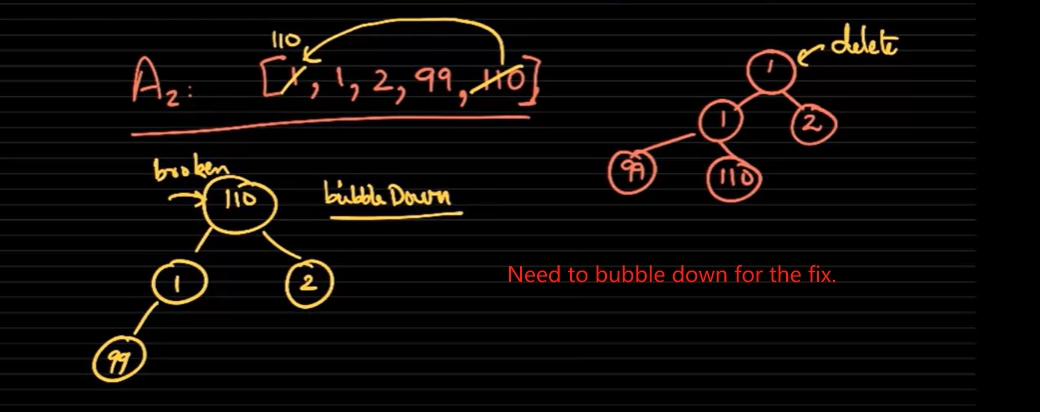
\includegraphics[width=\textwidth]{bubbledownafterdeletion.png}
\caption{Bubble down for a fix.}
\end{figure}

\paragraph{Here is a question regarding the fix operation after deletion of a heap.\\}


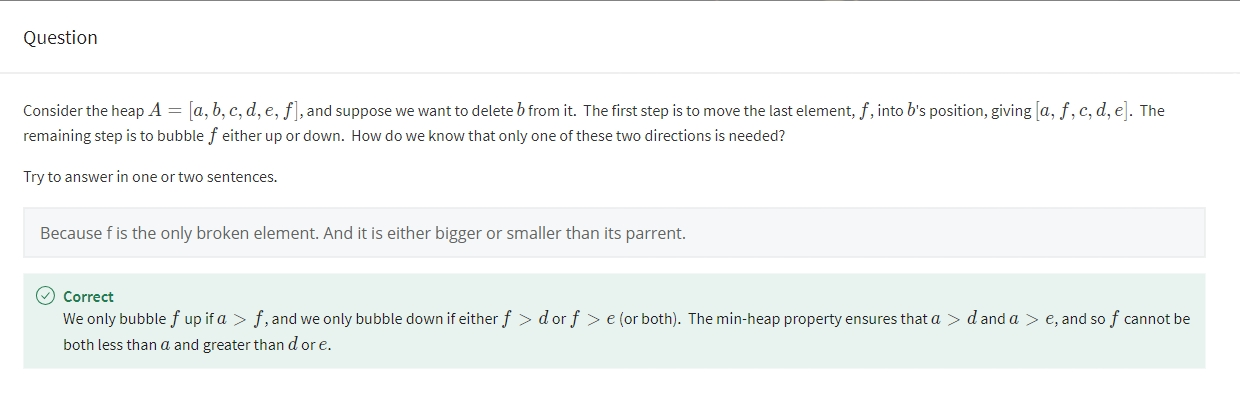
\includegraphics[width=\textwidth]{questionofdeletion.png}



\paragraph{The cost of time for deletion consists of two parts, 1 swap and then 2 bubble up/down.\\
The time of cost is $\theta(1)$ for step 1 and $\theta(\log_2^n)$ for step 2.\\
The total time cost is $\theta(\log_2^n)$.\\}


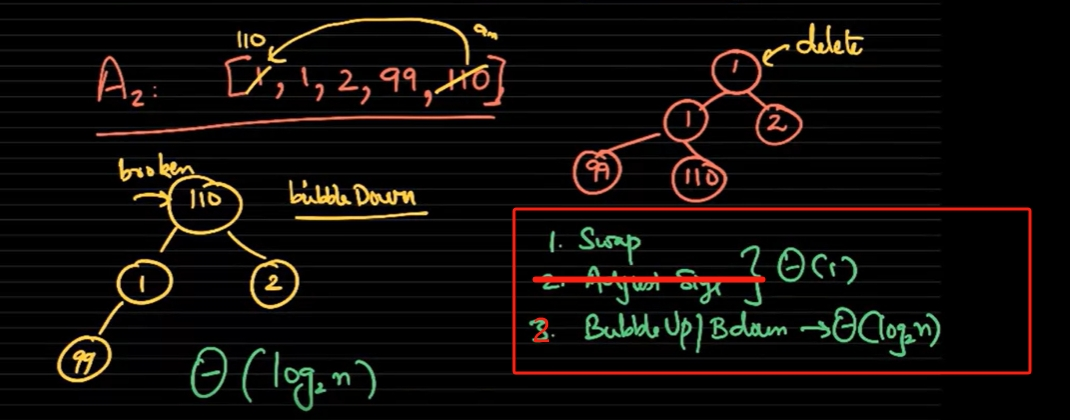
\includegraphics[width=\textwidth]{deletiontimecost.png}



\subsubsection{Finding the smallest element of a heap}

\paragraph{The time cost of finding the smallest element of a min heap is $\theta(1)$.\\
However, finding the largest element of a min heap is pretty hard and inefficient.\\}

\paragraph{Now we are talking about priority queue.\\
Priority queue is a data structure that will allow us to insert elements and delete the smallest one.\\
The main idea of priority queue is to keep the smallest element at the root of the heap.\\
Priority queue has a priority setting.\\}

\paragraph{We can bubble down elements that are in the wrong position and then get a min heap.\\
This is the main idea of heapify.\\
The running time of heapify is $O(n\log_2^n)$.\\}


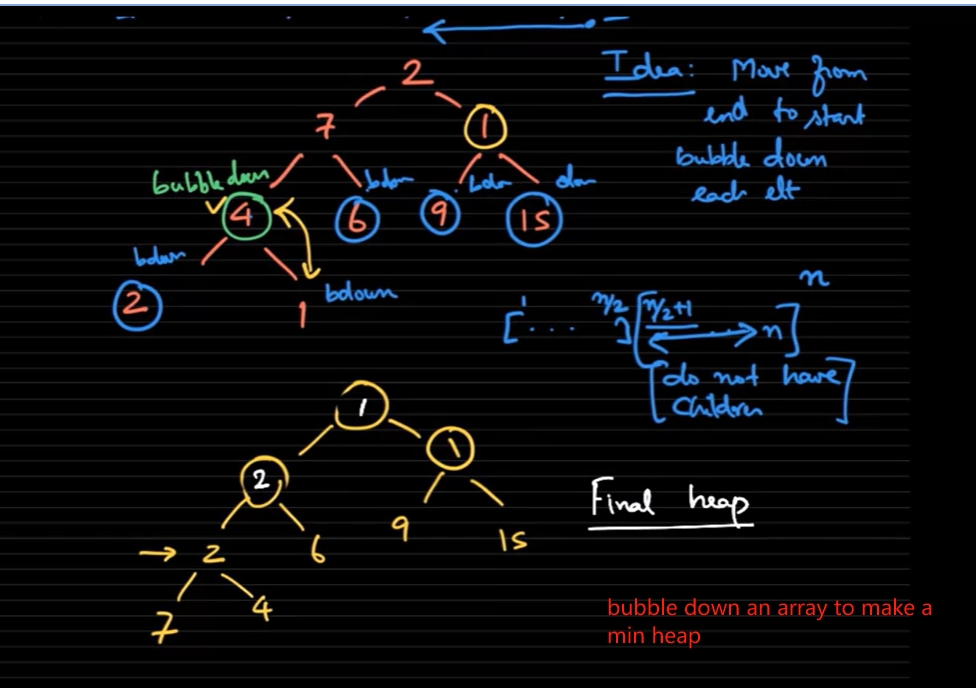
\includegraphics[width=\textwidth]{array2minheap.png}
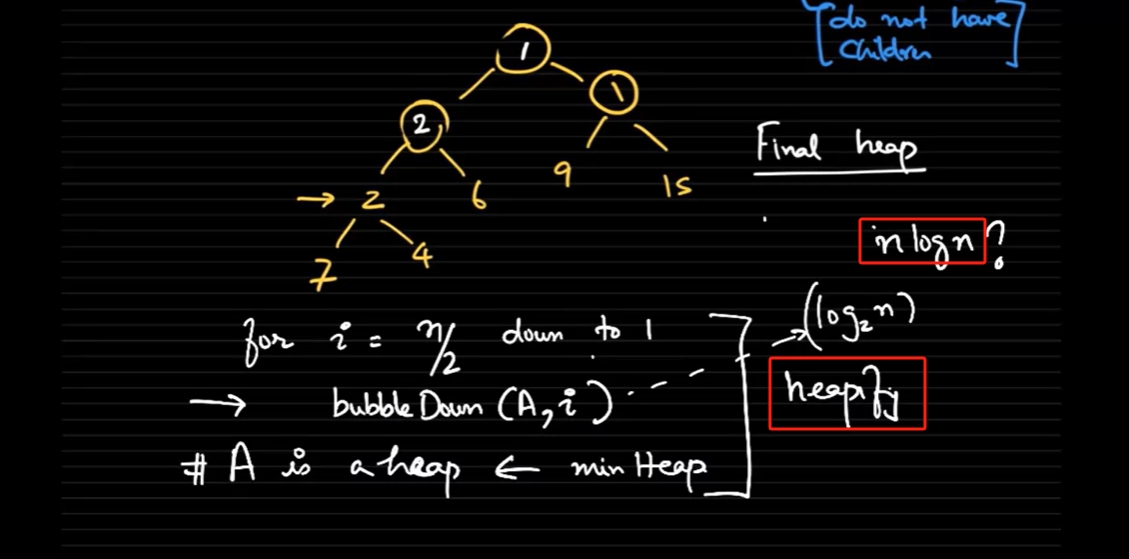
\includegraphics[width=\textwidth]{heapify.png}



\paragraph{The overall running time of heapify is linear to the size of the array. That is to say, the running time is $\theta(n)$.\\}


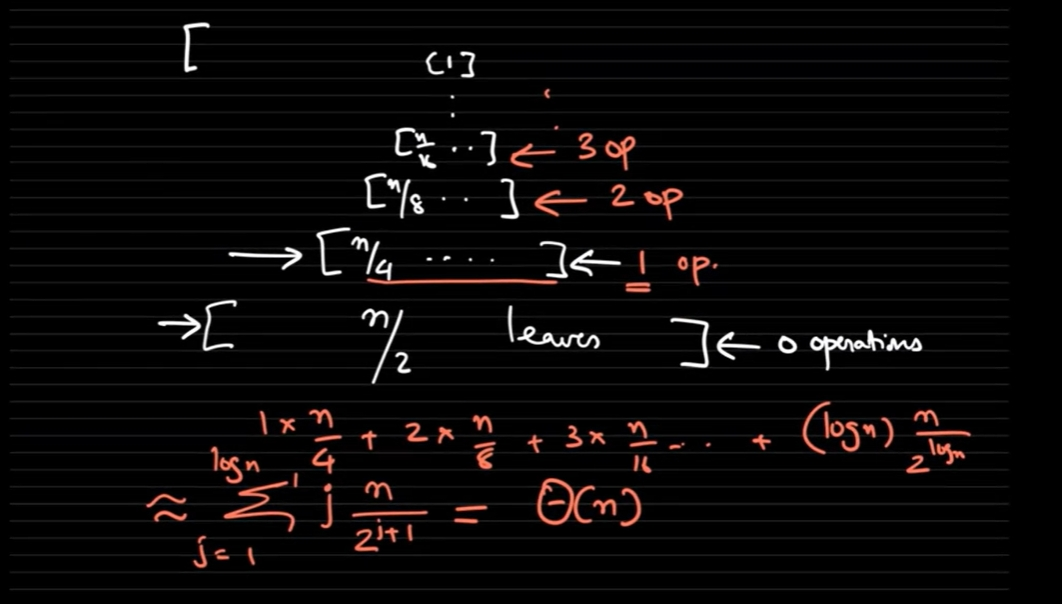
\includegraphics[width=\textwidth]{heapifyrunningtime.png}



\subsubsection{Heapsort}

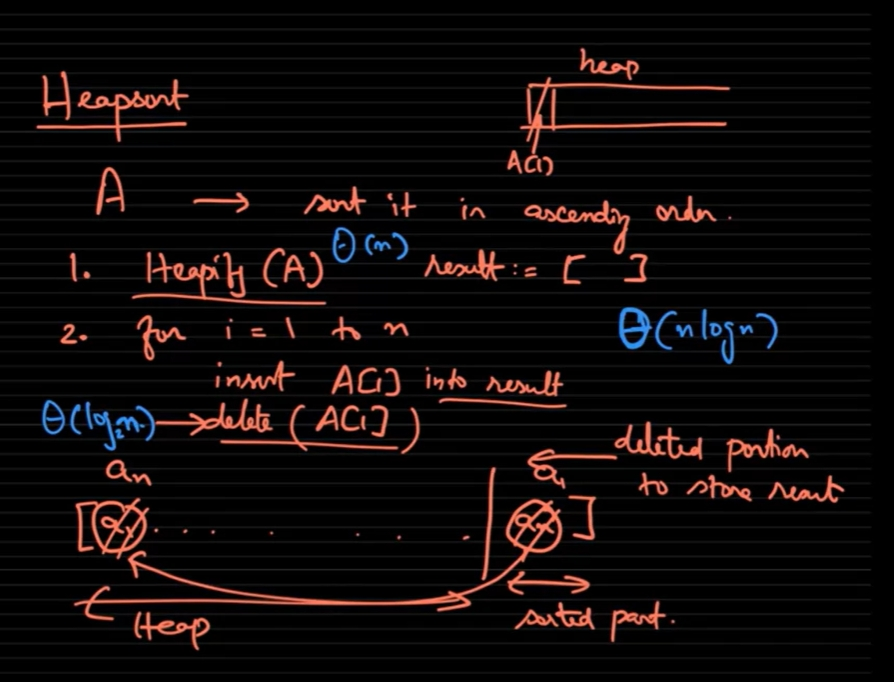
\includegraphics[width=\textwidth]{heapsort.png}
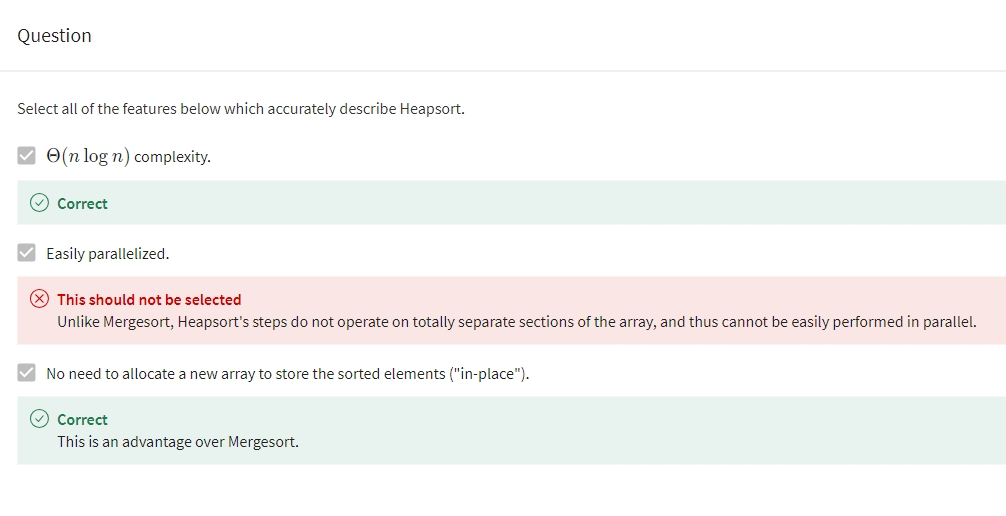
\includegraphics[width=\textwidth]{questionofheapsort.png}


\subsection{Quiz: Bubble-Up/Down, Insertion and Deletion}

\subsubsection{Question 1}


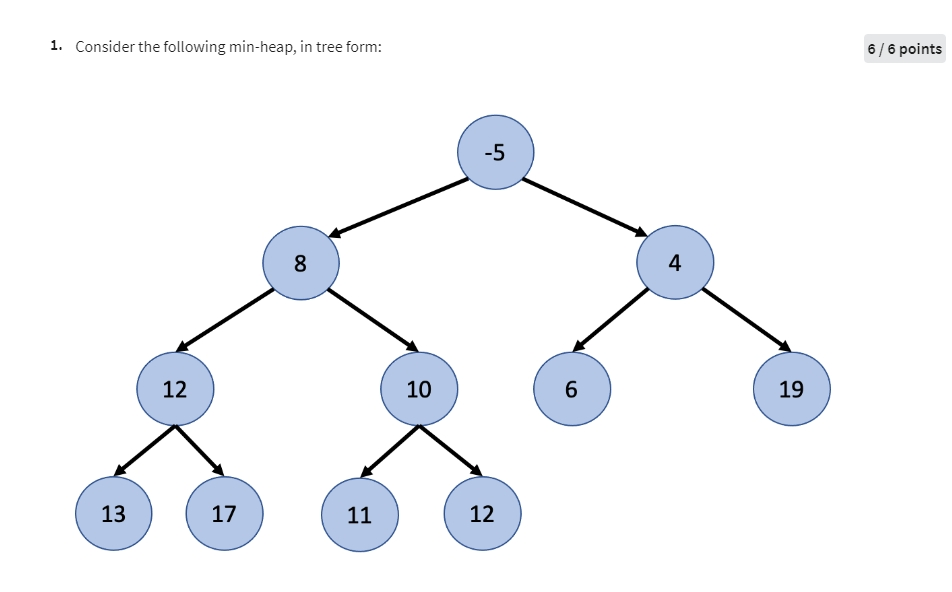
\includegraphics[width=\textwidth]{heapsortquestion1chart.png}



Consider the following min-heap, in tree form:\\
Now suppose we perform a heap-insert to add a new element 1 to the heap.Select all the correct facts about this insertion process from the list below.\\

The first step is to place the new element at the beginning of the array, making it the root of the tree.\\

\textcolor{red}{The first step is to place the new element at the end of the array, making it a child of the element.\\
Correct: After taking the first step, in which the new element is placed in the array, the heap property continues to hold.\\}

\textcolor{red}{In order to fix a heap property violation encountered during insertion, we perform a bubble-up operation, which swaps the new element and its parent element.\\
Correct: In order to fix a heap property violation encountered during insertion, we perform a bubble-down operation which swaps the new element with one of its child elements.\\}

When we insert 1 into the above min-heap, the first bubble-up step swaps element 1 with its parent 6.  This fixes all the min-heap property violations.\\

\textcolor{red}{When we insert 1 into the above min-heap, a second bubble-up step occurs which swaps element 1 with 4.  This fixes all the min-heap property violations.\\
Correct: This is correct.\\}

\textcolor{red}{In the worst case, bubbling up will require $\theta(\log_2^n)$ swaps, moving the inserted element all the way from a leaf position in the heap to the root.\\
Correct: This is correct: note that the length of the longest path from any leaf of a heap to the root is  at most $\log_2^n$.\\}


\subsubsection{Question 2}


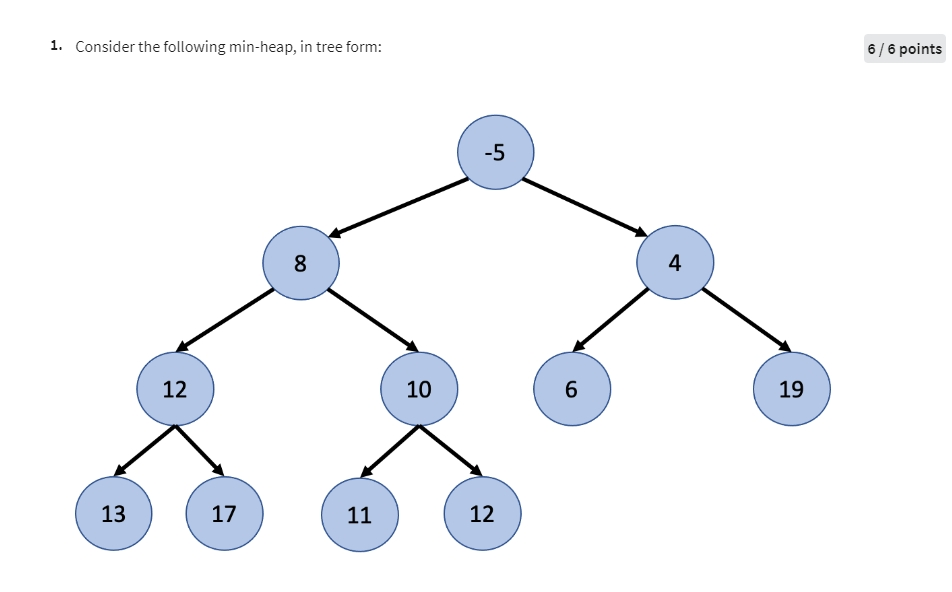
\includegraphics[width=\textwidth]{heapsortquestion1chart.png}



Consider again the min-heap example:\\
Suppose we heap-delete the element 8.\\

Select all correct facts about this deletion process from the list below.\\

\textcolor{red}{The first step replaces the element to be deleted (8) with the very last element in the heap's array (12).\\}

The first step replaces the element to be deleted (8) with the very first element in the heap's array (-5).\\

\textcolor{blue}{After the first step, in which we replace the element we are deleting (8), we are guaranteed that we have created at most one min-heap property violation.\\
This should be selected as well.\\}

\textcolor{red}{To fix the heap property violation caused by the first step, we perform a bubble-up or bubble-down operation depending on whether the swapped-in element is larger than its children or smaller than its parent.\\}

\textcolor{red}{Deletion of an element in a heap with n elements requires at $O(\log_2^n)$ comparison and swap operations.\\}


\subsection{Quiz: Heapify, Priority Queue and Heapsort}


\subsubsection{Question 1}

Suppose we wished to heapify  an array into a minheap using the following algorithm (assume $a[0]$ is not used and assume that bubble up routine is implemented).\\

\begin{verbatim}
def heapify (a):
    n = len (a)
    for i in range (1, n):
        bubble_up (a, i)
    return a
\end{verbatim}

\textcolor{red}{The worst case complexity of this procedure will be $\theta(n\log_2^n)$.\\}

\textcolor{red}{The procedure above is computationally less efficient than the one presented in the lecture because $n/2$ of the elements in the array may potentially need to bubble up all the way to the root.\\
Correct: Indeed: each of these $n/2$ elements may incur a cost proportional to $\log(_2^n)$ since they may each bubble up from the leaf to the root of he heap.\\}

Sorting the array using insertion sort will achieve the same complexity as the heapify procedure above. \\

\textcolor{red}{Sorting the array using mergesort will achieve the same complexity as the heapify procedure above.\\}

\textcolor{red}{The worst case of the procedure above is realized if we tried to heapify an array that is already sorted in descending order.\\}

The  worst case of the procedure above is realized if we tried to heapify an array that is already sorted in ascending order.\\

\subsubsection{Question 2}

Select all the facts that are true about the heapsort procedure in comparison with the insertion and mergesort procedures we have studied thus far. 
Assume that all heaps are minheaps unless otherwise mentioned in the option.\\

Heapsort requires extra storage to store the heap unlike insertion sort that can sort an array in place.\\

Heapsort is asymptotically faster than mergesort.\\

\textcolor{red}{If an array is already sorted in ascending order and the heapify procedure is run on it, then it does not modify the array in any way.} \\

If a min-heap is in fact already sorted in ascending order, deleting the minimum element operation runs in constant time.\\



\section{Hashtables}

\paragraph{The basic idea of hashtables is to implement a mapping from keys to values.\\
What's important of a hashtable is not key or value, but a special function called hash function.\\
With the hash function implemented, the key will be converted to a hash value.\\
The hash value will be used as an index to store the value. That is to say, the key will be converted to an index. However, since the hash value is based on the key itself,
different keys may have the same hashed values, which means the same index may be mapped with several keys. How do we deal with this?\\}

\subsection{Chaining for Collision Resolution}

\paragraph{The chaining of a hashtable is to store all the values that have the same index in a linked list. This list is empty initially.\\
When we insert a new key-value pair, we will first calculate the hash value of the key. Then we will check if the index is empty. 
If it is, we will simply insert the key-value pair. If not, we will insert the new pair to the linked list.\\}

\paragraph{If we want to delete, we will first calculate the hash value of the key. Then we will check if the index is empty. If it is, we will simply delete the key-value pair. 
If not, we will delete the key-value pair from the linked list.\\}

\subsection{Load Factor}

\paragraph{The load factor is the ratio of the number of key-value pairs to the number of indices. Suppose we have $m$ slots(indices) and $n$ key-value pairs.
The load factor is $n/m$.\\}


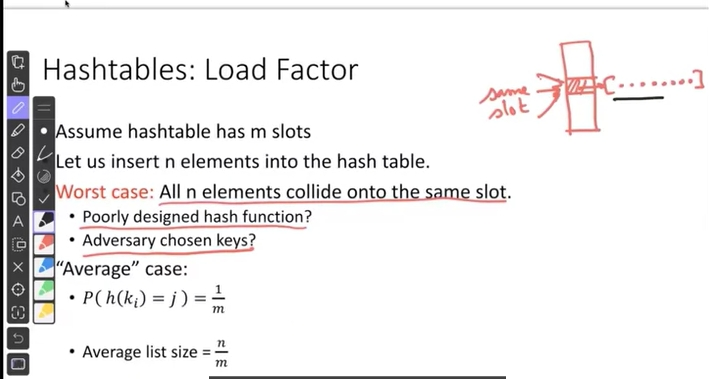
\includegraphics[width=\textwidth]{hashtableloadfactor.png}


\subsection{Rehashing}

\paragraph{Rehashing is the process of creating a new hashtable with a larger number of slots. 
Since we need to go through all the key-value pairs (n pairs) and all the slots/indices (m slots) in the original hashtable in order to create the new one,
The running time of rehashing is $O(n+m)$.\\}


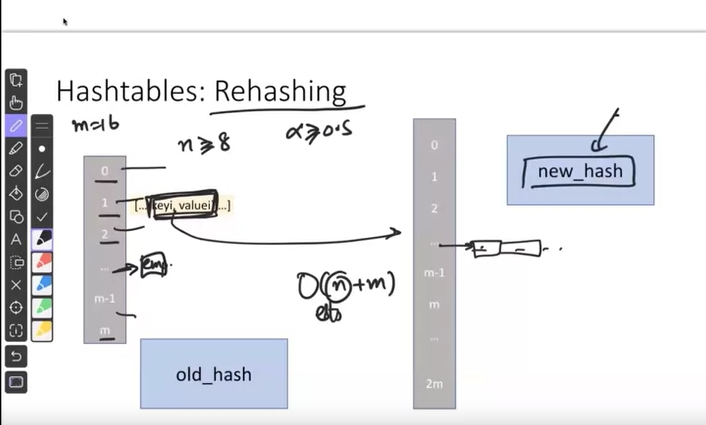
\includegraphics[width=\textwidth]{hashtablerehashing.png}


\subsection{Quiz: Hashtables}

\subsubsection{Question 1}

Select all true facts about Hashtables which use unordered-list chaining to resolve collisions.\\


Given a Hashtable with m slots and containing n elements, the average number of elements chained together on a single slot is $m*\log_2^n$.\\


\textcolor{blue}{The Find operation, which returns a value for a key if it is present in the Hashtable, has a worst-case complexity of $O(n)$ for a table containing n entries.\\}


The cost of the hash function depends on the number of elements currently stored in the table.\\


\textcolor{red}{Expanding the number of slots in a Hashtable requires re-applying a hash function to every element already stored.\\}

Given a Hashtable with m slots and containing n elements, the average number of elements chained together on a single slot is $n/m$.\\


\subsubsection{Question 2}

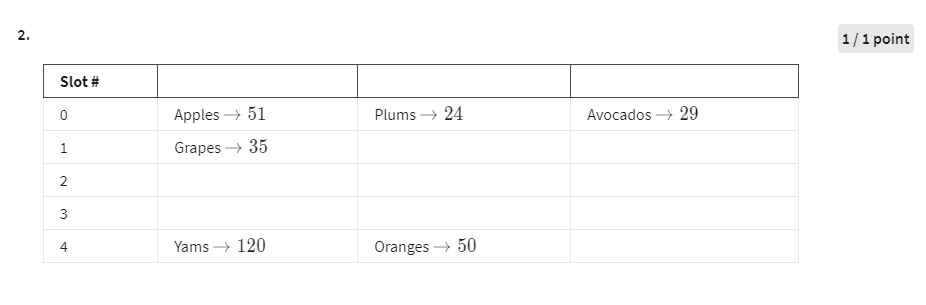
\includegraphics[width=\textwidth]{hashtablequestion2.png}

Consider the above Hashtable, which stores numbers for different produce items (maybe the amount in stock at a store) according to a hash function called HASH.\\

For the entry Apples →51, the key is Apples and the value is 51.  
The entry for Apples is at the front of a chained list including Plums and Avocados, which all share Slot 0.\\

The HASH function picks a slot for the entry by taking the ASCII value of the first letter of the key, mod 5. So for Apples, it is 
$65\bmod5=0$ You won't need to calculate these for this problem.\\

Suppose it costs 1 time unit to run HASH, and 1 time unit to check whether an entry is already present in each place in the chained lists.  
It also takes 1 time unit to write a new value to a particular place in a chained list.  
Assume that newly inserted items must go at the end of the chained list in their slot.\\


How many time units does it cost to insert a new entry Limes → 40 into the Hashtable?  When HASH is called on Limes, it gives $76 \bmod 5 = 1$.\\

Answer:3\\


\section{Introduction to Randomization, Average Case Complexity Analysis and Recurrences}

\paragraph{The topic of this section is Randomization in Algorithm and Data Structures.\\}

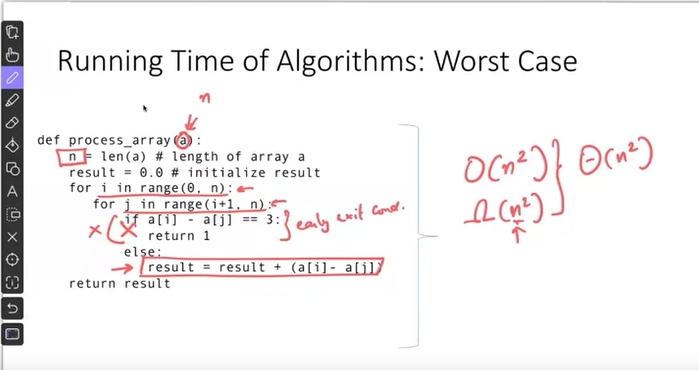
\includegraphics[width=\textwidth]{randomizationrunningtime.png}

\subsection{Algorithm that Use Randomness}

\paragraph{The main idea of randomization is to use randomness in the algorithm.\\
The main advantage of randomization is that it can reduce the running time of the algorithm, so
that we will focus on the average case of the running time rather than the worst case.\\
When looking at the running time of an algorithm, we typically consider the worst case scenario.\\
While in the case of randomization, the probability of worst case is relatively low because Of
the nature of randomness. Therefore, it is not efficient to always consider the worst case, since
it may not happen, and the average case of running time may be much lower and more realistic.\\}

\paragraph{Let's take a look at this $geometric(p)$ function.\\
We will introduce a new concept $T(p)$, which is the expected value of the geometric function, 
a unknown average case running time.\\}


\begin{figure}[h]
    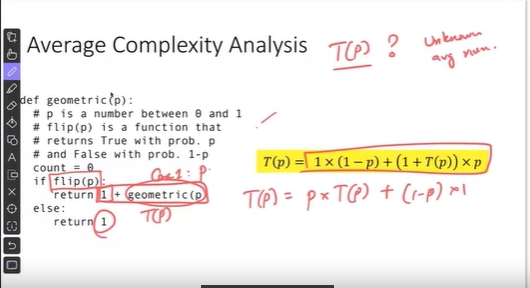
\includegraphics[width=\textwidth]{averagerunningtimetp.png}
    \caption{When running into case 1, a.k.a. $flip(p) == True$, the running time will be
    $p*(1+T(p))$, and in the other case, when $flip(p) == False$, the running time will be
    $1*(1-p)$.}
\end{figure}

\paragraph{
    The unknown running time $T(p) = p*(1+T(p)) + (1-p)*1$, which can be simplified to $T(p) = 1/(1-p)$.\\
}

\subsection{Analysis of Algorithms: Recurrences}

\paragraph{Here is a general understanding of recurrences.\\}

\begin{figure}[H]
    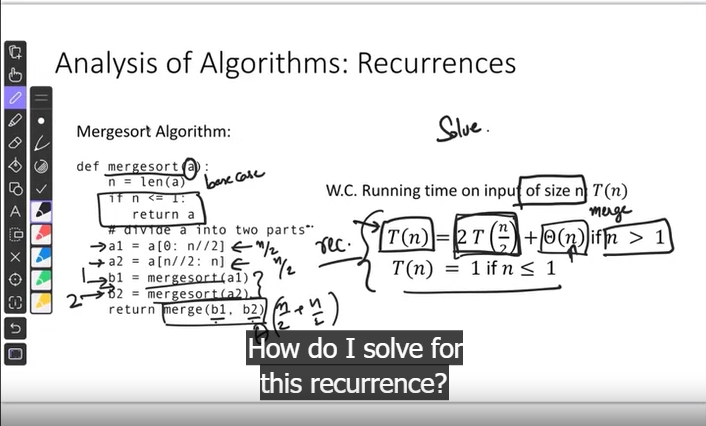
\includegraphics[width=\textwidth]{recurrencerelations.png}
    \caption{The $T(n)$ equation is a recursive function in this Mergesort function. 
    If $n<=1$, the function returns 1, where running time is 1. Otherwise, the function will be
    $2*T(n/2) + n$ based on the function details.\\}
    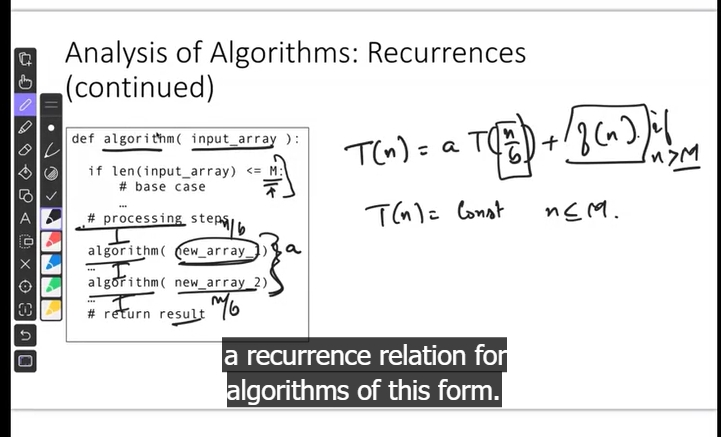
\includegraphics[width=\textwidth]{recurrencerelations2.png}
    \caption{Here is a general form of a recursive function. \\
    $T(n) = a*T(n/b) + \theta(n), if n > m$\\
    $T(n) = Constant, if n <= m$}
\end{figure}

\paragraph{If we want to solve for the recurrence relations, we can use the expansion method.\\
The main idea is to expand the function until we reach the base case.\\}

\begin{figure}[H]
    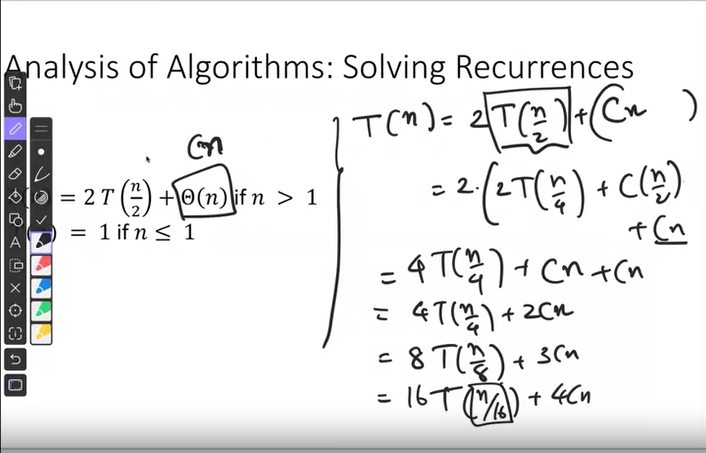
\includegraphics[width=\textwidth]{expansionmethod.png}
    \caption{We can assign $C(n) == \theta(n)$ at first.\\
    Then, we assign $T(n)$ to the original function with an expanded form.\\
    For example, by multiplying $2$, $T(n) = 2*T(n/2) + C(n) + D$ will be converted to $T(n) = 2(2T(n/4) + C(n/2) + D) + C(n) +D$.\\
    This expansion the function will keep going on by 4, 8 ,16 etc., until it reaches the base case, as displayed in the firgure.\\
    The running time of this function is $\theta(n^{\log_b^a})$.\\}
\end{figure}

\section{Partition and Quicksort Algorithm}

\subsection{Basic Idea and Pseudocode}

\paragraph{Quicksort is an efficient in-place sorting algorithm that uses the divide and conquer strategy.\\
Basically it divide the array into two parts, one with the elements smaller than the pivot and the other bigger.\\
At first glance, quicksort sounds a lot like mergesort, but the main difference is that in mergesort, the major time costing part is
 at the end of the function when merging is taking place; while in quicksort, we will conduct a lot of work by partitioning the array first.\\}

 \paragraph{What is the partition function?\\
 First we are going to choose a pivot element from within the array and it doesn't matter which one we choose.
 Then we will compare all the rest of the elements with the pivot and divide them into smaller-than-pivot and 
 larger-than-pivot part. At this stage, we are not necessarily sorting what is being compared.\\
 Now we get a updated array where the pivot is rested somewhere in the middle range of the array, and it is the final position for 
 the pivot in the fully sorted array later. All we need to do now is to sort the left part and the right part.\\}

\paragraph{Here is the pesudocode for quicksort. $left$ means the index of the first element in array $A$ and $right$ means the index of the last.\\}

\begin{verbatim}
    quicksort(A,left,right):
        #Base case
        if right-left <= 1:
            swap(A[left],A[right])
            return
        # First just choose a element as pivot.
        x == A[right]
        p = partition(A,x)
        # Then we call quicksort recursively.
        quicksort(A,left,p-1)
        quicksort(A,p+1,right)
\end{verbatim}

\subsection{Quiz on Quicksort}

\begin{figure}[H]
    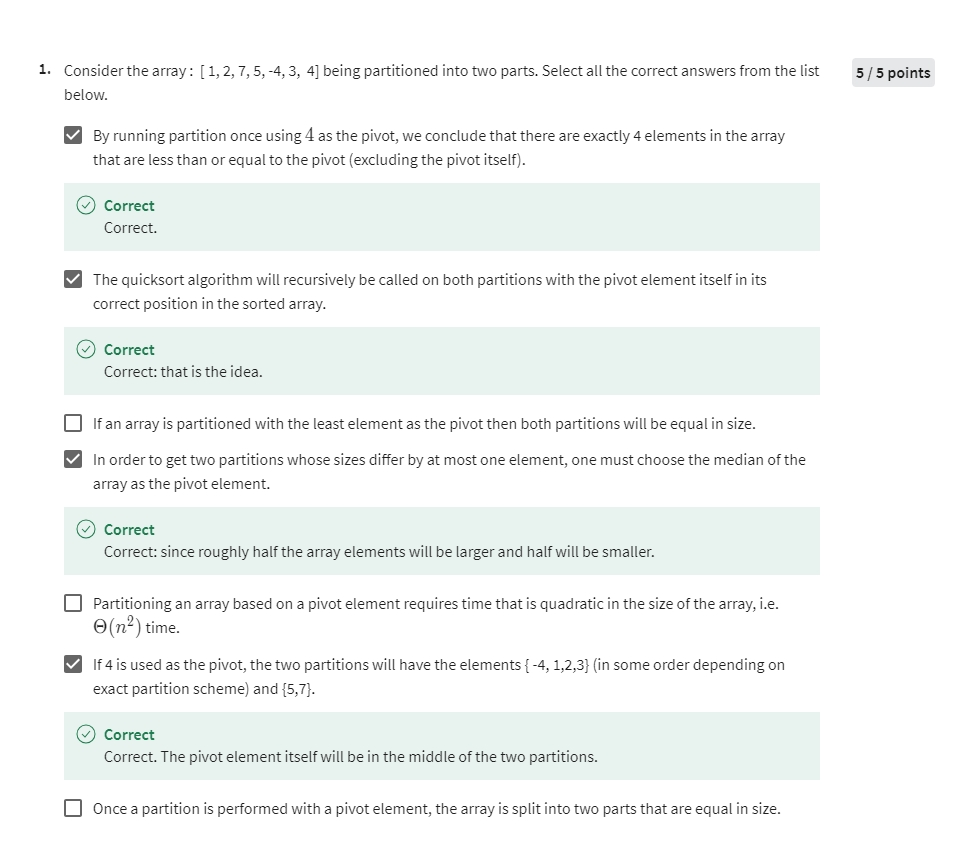
\includegraphics[width=\textwidth]{week3quicksortquiz1.png}
    \caption{Quiz 1\\}
\end{figure}

\begin{figure}[H]
    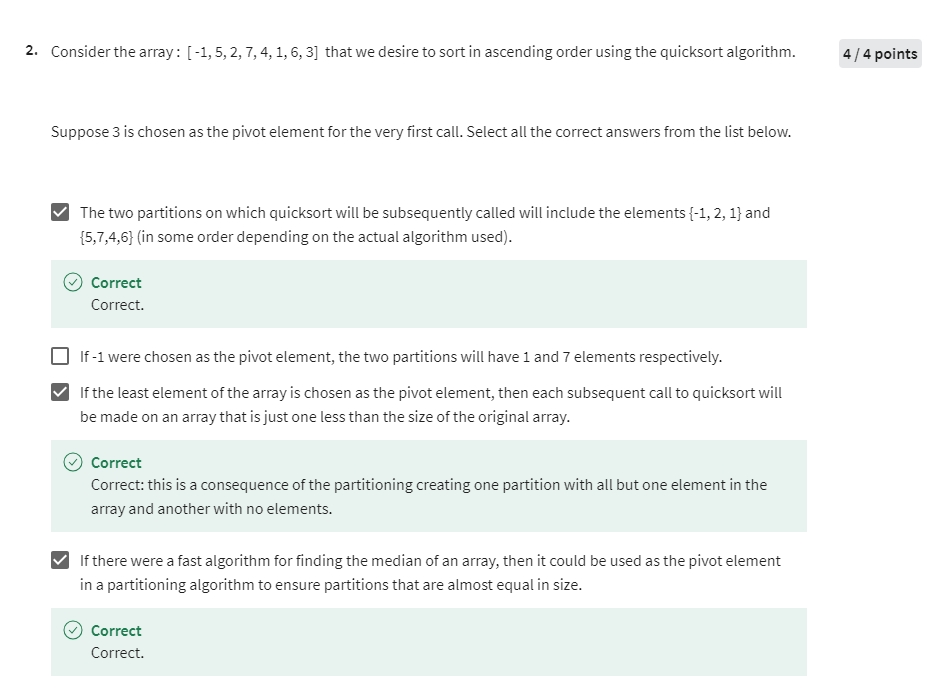
\includegraphics[width=\textwidth]{week3quicksortquiz2.png}
    \caption{Quiz 2\\}
\end{figure}

\section{Designing Partition Scheme and Correctness}

\paragraph{First we will go through the Lomuto Partition Scheme.\\
We will introduce two intermediate variables, $i$ and $j$, which are the index of the first element 
and the last element of the array.\\
Then we will choose the last element as the pivot.\\
The original array can be divided into four parts, 
$A[1, \ldots ,i-1], A[i, \ldots ,j-1], A[j, \ldots ,n-1], A[n]$.\\
The end of the first region can be either $i$ or $i-1$ as noted, which is not a big deal.\\
The main idea of the Lomuto Partition Scheme is to compare the element at index $j$ with the pivot.\\
If the element is smaller than the pivot, we will swap it with the element at index $i$ and then increase $i$ by 1.\\
That is to say, everything after $j$ is categorized as ``unprocessed''.}

\paragraph{Here is a step-by-step analysis of the partition scheme.\\
Let $i=0, j=1$, and the pivot is $x = A[n]$.\\
Under this situation, everything besides the pivot is unprocessed, located in Region 3.\\
$\forall Region1 < x$, $\forall Region2 >= x$,\\
if $A[j] < x$, we will swap $A[i]$ and $A[j]$, and then increase $i$ as well as $j$ by 1.\\
If $A[j] >= x$, we will do nothing but increasing $j$ by 1.\\
Here is the pseudocode for the Lomuto Partition Scheme.\\}

\begin{verbatim}
    partition(A,x):
        # Four regions: A[1,...,i-1], A[i,...,j-1], A[j,...,n-1], A[n]
        i = 0
        j = 1
        # Perform partitioning until the end of the array.
        while j <= n-1:
            if A[j] < x:
                swap(A[i],A[j])
                i += 1
                j += 1
            else:
                j += 1
        # Swap and place the pivot to its right position.
        swap(A[i],A[n])
        return i
\end{verbatim}

\paragraph{The running time of Lomuto Partition Scheme is just $n$.\\}

\subsection{Lomutio Partition Algorithm Quiz}

\begin{figure}[H]
    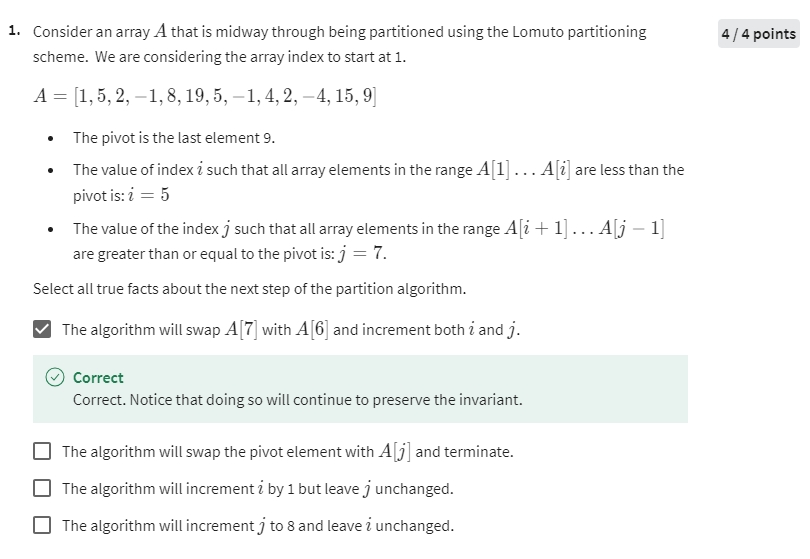
\includegraphics[width=\textwidth]{week3lomutoquiz1.png}
    \caption{Quiz 1\\}
\end{figure}

\begin{figure}[H]
    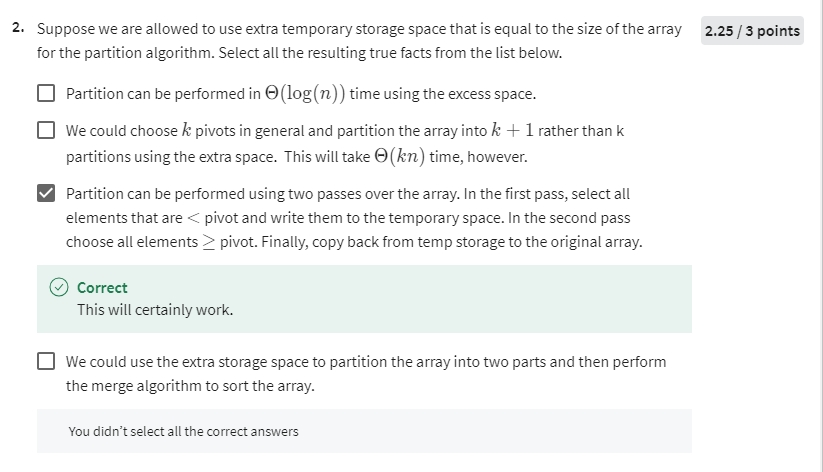
\includegraphics[width=\textwidth]{week3lomutoquiz2.png}
    \caption{Quiz 2\\}
\end{figure}

\section{Analysis of Quicksort Alogorithm}

\paragraph{The best case analysis of quicksort is that what we call a balanced partition.\\
Although it rarely happens, the running time when occuring is $\theta(nlog^n)$.}

\paragraph{Now Let's take a look at the worst case analysis of quicksort algorithm.\\
The worst case of quicksort is when the pivot is the smallest or the largest element of 
the array. Therefore, either side of the pivot will be empty.\\
The running time of the worst case is $\theta(n^2)$, which equals to the running time of insertion sort.\\
So what we should do is to avoid the worst case by choosing a pivot randomly.\\
The expected running time of quicksort is $\theta(nlog^n)$.\\}

\begin{figure}[H]
    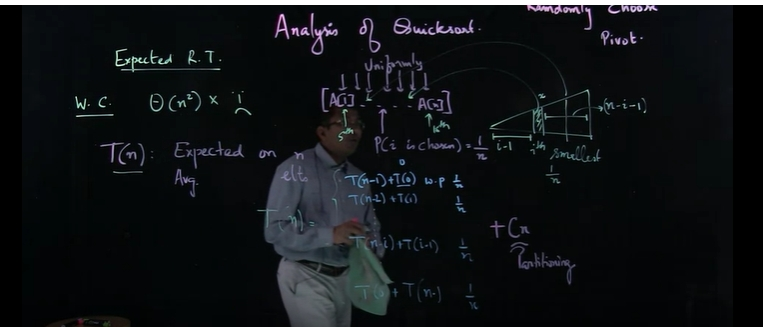
\includegraphics[width=\textwidth]{expectedaveragerunningtime.png}
\end{figure}

\paragraph{Let's assume $T(n)$ is the expected (or average) running time of quicksort.\\
Here is the equation of $T(n)$.\\
$T(n) = 1/n [\sum_{i=1}^{n-1} T(i) + \sum_{i=1}^{n-1} T(n-i)] + n$\\
And it equals to\\
$T(n) = 2/n [\sum_{i=1}^{n-1} T(i)] + n$\\
The above is the compressed form of the equation. We can expand it like the following;\\
$T(n) = 2/n [T(1)+T(2)+ \cdots + T(n-1)] + n$.\\
If we multiply $n$ on both sides, we get\\
$n*T(n) = 2[T(1)+T(2)+ \cdots + T(n-1)] + n^2$.\\
If we replace $n$ with $n-1$, we will get\\
$(n-1)*T(n-1) = 2[T(1)+T(2)+ \cdots + T(n-2)] + (n-1)^2$.\\
Then we can subtract $nT(n-1)$ from $nT(n)$ and get\\
$nT(n) - (n-1)T(n-1) = 2T(n-1) + 2n - n^2 + n - 1$.\\
$T(n) = T(n-1) + 1/nT(n-1) + 2 - 1/n$.\\
Now once again, we will try to expand the above equation.\\
For convenience, we will assume $2-1/n = \theta(1)$.\\
Then we will get $T(n) = T(n-1) + \theta(1)$\\
$T(n) = T(n-1) + \theta(1)$\\
$T(n) = T(n-2) + 2\theta(1)$\\
$\cdots$
$T(n) = (n+1)/(n-j+1)T(n-j) + \sum_{i=1}^{j-1} (n+1)/(n-i)*2\theta(1) + \theta(1)$.\\
When $j == n$, the equation will be\\
$T(n) = \sum_{i=1}^{j-1} (n+1)/(n-i)*2\theta(1) + \theta(1)$.\\
$T(n) = [(n+1)/n + (n+1)/(n-1) + \cdots + (n+1)/1]*2\theta(1) + \theta(1)$\\
$T(n) = 2\theta(1)[n+1][1 + 1/2 + 1/3 + \cdots + 1/n] + \theta(1)$\\
The above equation is the harmonic series, in which the $1 + 1/2 + 1/3 + \cdots + 1/n$ part is called the nth harmoic number, 
and it equals to $\theta(\log^n)$.\\
Therefore, $T(n) = 2\theta(1)\theta(\log^n)$,\\
Then we can get the final result of $T(n) = nlog^n$, a.k.a $\theta(n\log^n)$.
Now we can say, if we choose a pivot randomly in Quicksort, the average running time will be $\theta(n\log^n)$.\\}

\subsection{Quiz on Quicksort Analysis}

\begin{figure}[H]
    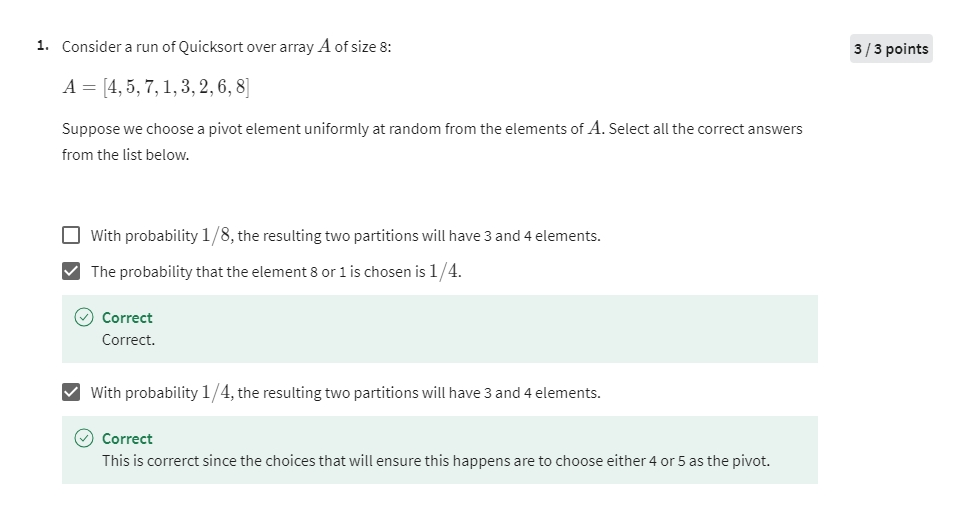
\includegraphics[width=\textwidth]{quicksortanalysisquiz1.png}
    \caption{Quiz 1\\}
\end{figure}

\begin{figure}[H]
    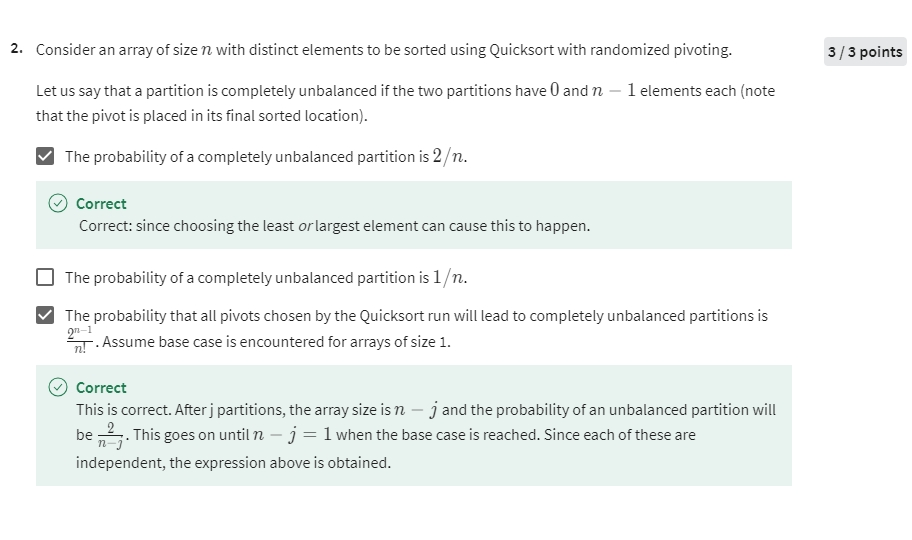
\includegraphics[width=\textwidth]{quicksortanalysisquiz2.png}
    \caption{Quiz 2\\}
\end{figure}

\begin{figure}[H]
    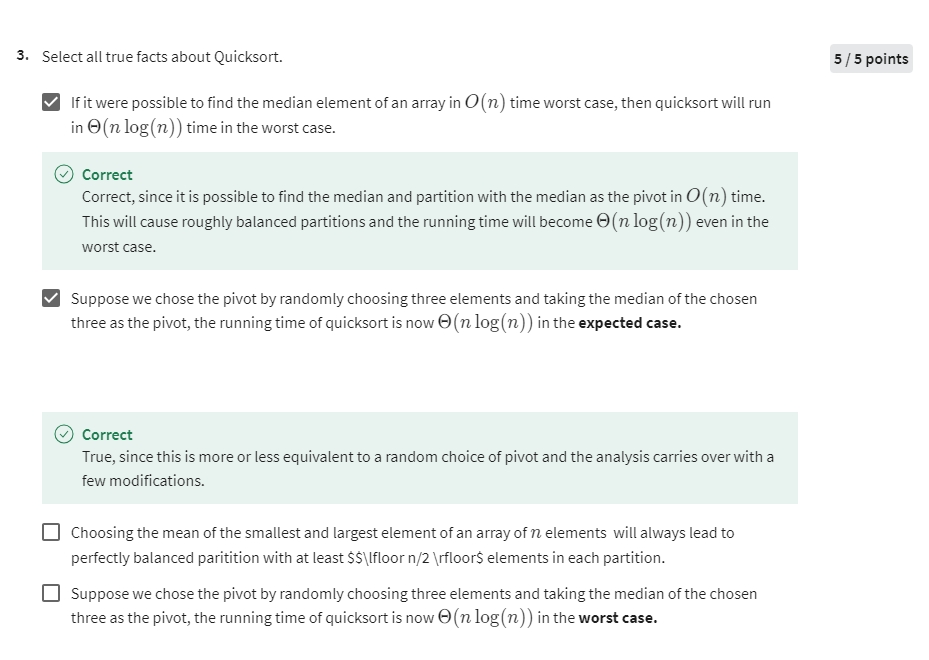
\includegraphics[width=\textwidth]{quicksortanalysisquiz3.png}
    \caption{Quiz 3\\}
\end{figure}


\section{Quickselect Algorithm}

\paragraph{The main idea of Quickselect is to find the kth smallest element in an array.\\
We can use Quicksort to select better than the brute force method, which is just trying to
sort the array first and then find the target by comparing every element.\\
The running time of the brute force method is $\theta(n\log^n)$, 
while the running time of Quickselect is $\theta(n)$.\\
Here is the logic of using quicksort for quckselect function.\\
At first, we will choose a pivot and partition the array.\\
Then we will compare the pivot with the target.
Let's say the pivot is j in array A with n elements in total.\\
If $j == k$, we will return the pivot.\\
If $j > k$, we will recursively call quickselect on the left part of the pivot,
a.k.a. $quickselect(A[1], \ldots ,A[j-1])$.\\
If $j < k$, we will recursively call quickselect on the right part of the pivot,
a.k.a. $quickselect(A[j+1], \ldots ,A[n])$.\\}

\begin{figure}[H]
    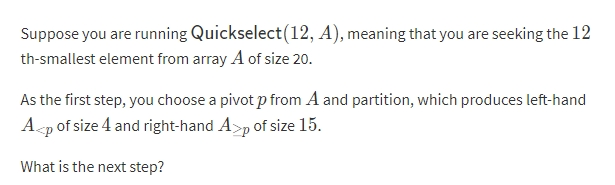
\includegraphics[width=\textwidth]{quickselectlittlequiz.png}
    \caption{The next step will be to perform a $quickselect(12-5,A>=p)$ operation,
    in order to find the $7th$ smallest element on the right side of the pivot,
    since the $12th$ smallest element is already larger than the 4 elements
    in the left side of the pivot.\\}
\end{figure}

\paragraph{Now let's go through a real example of quickselect.\\
Let's say we have an array $A = [3,2,1,5,4,6,7,8,9]$.\\
We want to find the 4th smallest element in the array.\\
Let's say we choose the pivot randomly and it's 5.\\
After partitioning, the array will be $A = [3,2,1,4,5,6,7,8,9]$.\\
The pivot is 5, which is the 5th smallest element. Since pivot > k,
we need to focus on the left side of the pivot, which is $[3,2,1,4]$.\\
Now we need to find the 4th smallest element in the left side of the pivot.\\
Let's say we choose the pivot randomly and it's 2.\\
After partitioning, the array will be $A = [1,2,3,4]$.\\
The pivot is 2, which is the 2nd smallest element. Since pivot < k,
we need to focus on the right side of the pivot, which is $[3,4]$.\\
Since the 4th smallest element is already larger than the 2 elements 
in the left side of the pivot, we can just find the $4-2=2th$ smallest elment in
$[3,4]$, which is 4.\\}

\begin{figure}[H]
    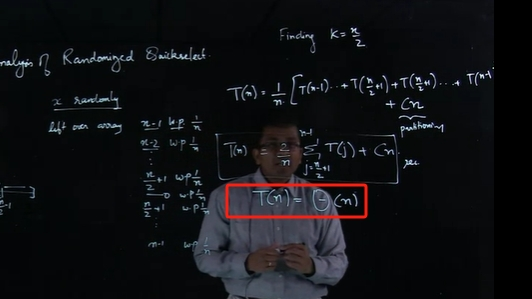
\includegraphics[width=\textwidth]{quickselectrunningtime.png}
    \caption{The running time of $T(n)$ is actually $\theta(n)$.\\}
\end{figure}

\subsection{Quiz on Quickselect}

\begin{figure}[H]
    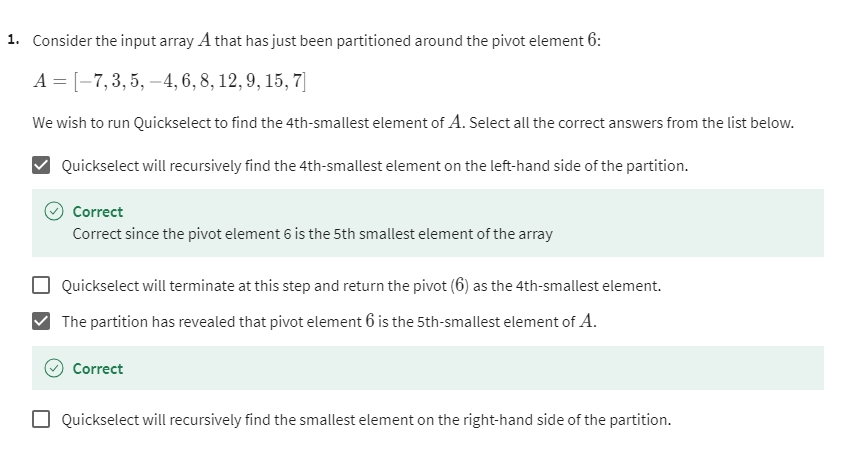
\includegraphics[width=\textwidth]{quickselectquiz1.png}
    \caption{Quiz 1\\}
    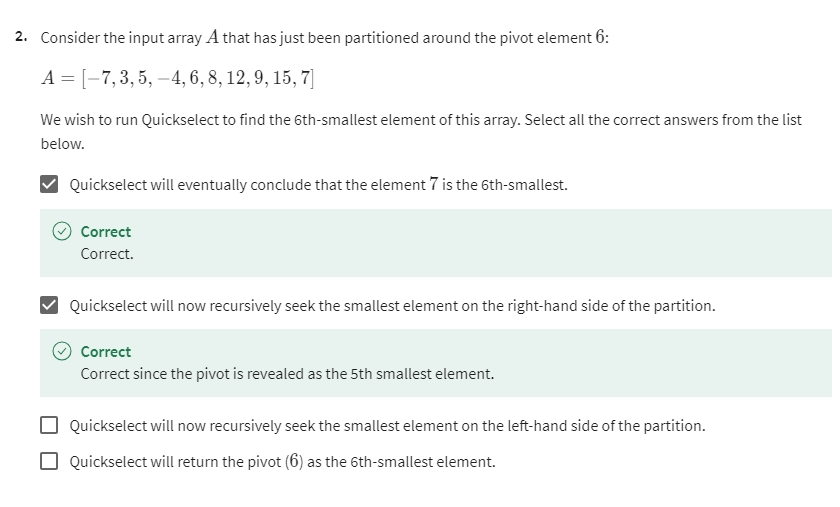
\includegraphics[width=\textwidth]{quickselectquiz2.png}
    \caption{Quiz 2\\}
    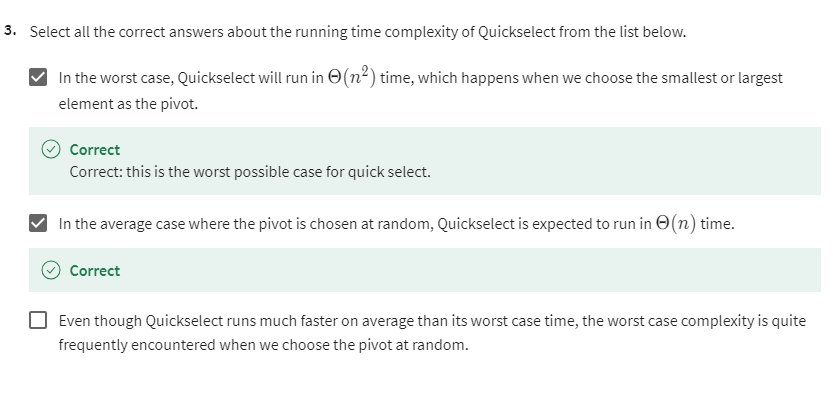
\includegraphics[width=\textwidth]{quickselectquiz3.png}
    \caption{Quiz 3\\}
    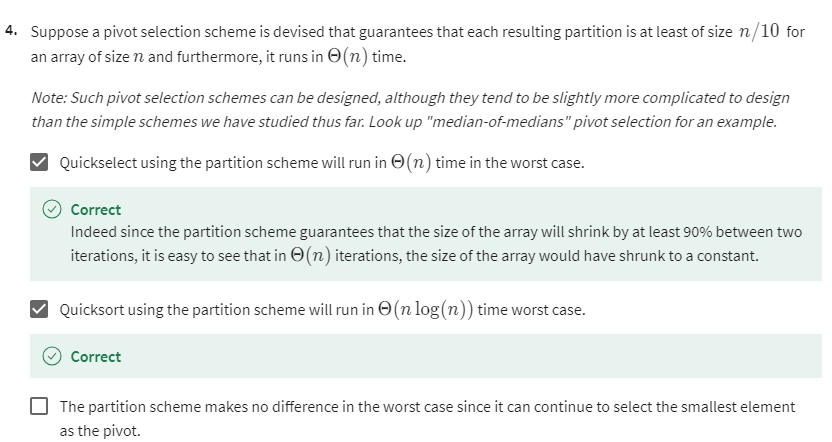
\includegraphics[width=\textwidth]{quickselectquiz4.png}
    \caption{Quiz 4\\}
\end{figure}































\end{document}